\chapter{Method C: knowledge-driven analysis}
\chaptermark{Knowledge-driven analysis}
\label{chap:knowledge}
\graphicspath{{./chapters/5-knowledge/figs/}}

Document image analysis is an active field of research which can attain a complete understanding of the semantics of a given document.
One example of the document understanding process is enabling a computer to understand a comic strip story.
In this chapter we propose a knowledge-driven system that can interact with bottom-up and top-down information to progressively understand the content of a document.
We also model the comic book's and the image processing domains knowledge for information consistency analysis.

%----------------------------------------------
% Introduction
\section{Introduction}
\label{sec:kn:introduction}

\modif{
  Nous introduisons dans ce chapitre les ontologies développées pour l'analyse automatique de bandes dessinées.
Nous progressons en plusieurs étapes.
Tout d'abord, nous présentons une première ontologie formalisant les notions relatives au traitement d'images, le type de données, les entrées, les sorties et  l'évaluation des résultats.
Dans un deuxième temps, nous déroulons le processus de conceptualisation du domaine de la bande dessinée, pensée pour être utilisée dans un contexte d'analyse d'images.
Enfin, nous expliquons comment ces ontologies communiquent l'une avec l'autre, afin de pouvoir être utilisées conjointement.
}

In this chapter we address the problem of understanding comics by automatically improving the consistency of the extracted elements according to the domain knowledge and by inferring new information and launching further processing iteratively.
Detecting these elements and establishing their relationship is crucial towards complete comics understanding.
Low level and high level information is used in a complementary and unsupervised way, to progressively identify the different elements of a digitized comic book image and their semantic relations (Figure~\ref{fig:kn:intro_illustration}).

%%%%%%%%%%%%%%%%%%%%%%%%%%%%%%%%%%%%%%%%%%%%%%%%%%%
 \begin{figure}[ht]  %trim=l b r t  width=0.5\textwidth,
   \centering
  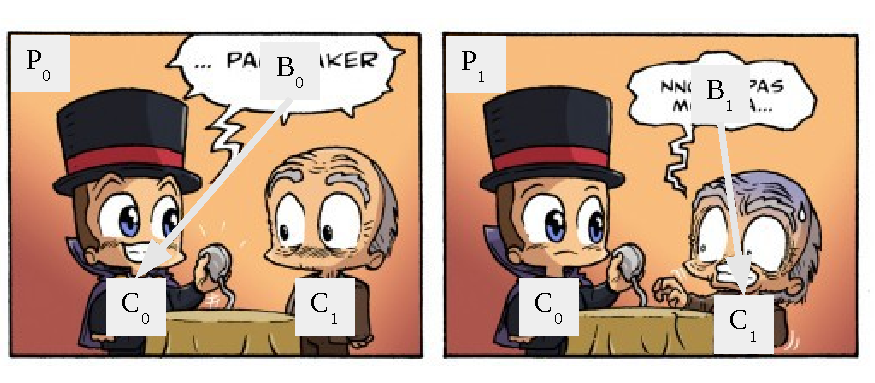
\includegraphics[trim= 0px 10px 3px 10px, clip, width=0.5\textwidth]{intro_illustration.pdf}
  \caption{The left panel $P_0$ represents a comics character labelled as $C_0$ saying the content of balloon $B_0$ to another character labelled as $C_1$. In the right panel $P_1$, the character $C_1$ is saying $B_1$ to $C_0$.}
  \label{fig:kn:intro_illustration}
 \end{figure}
%%%%%%%%%%%%%%%%%%%%%%%%%%%%%%%%%%%%%%%%%%%%%%%%%%%


The proposed framework is based on interactions between low and high level processing in order to reduce the challenging semantic gap.
%Here, the different level of information are given by an image processing and an expert system respectively. 
We call each image processing algorithm an ``extractor'' of panels, balloons (or bubbles), tails and comic characters (protagonists) according to the type of region they are designed for.
Extractors provide a set of regions that feeds a knowledge base.
%in the different extraction processes such as panel and speech balloon improvements and validation (e.g. panel, text, speech balloon) and their combination to guide other feature extractions (e.g. person object).
The knowledge base is associated with rules that form an ontology.
The main difficulty is to extract but also to model the diversity of styles, format, definition and the differences between design and printing techniques (Figure~\ref{fig:kn:comics_diversity}).

%%%%%%%%%%%%%%%%%%%%%%%%%%%%%%%%%%%%%%%%%%%%%%%%%%
\begin{figure}[ht]  %trim=l b r t  width=0.5\textwidth,
   \centering
  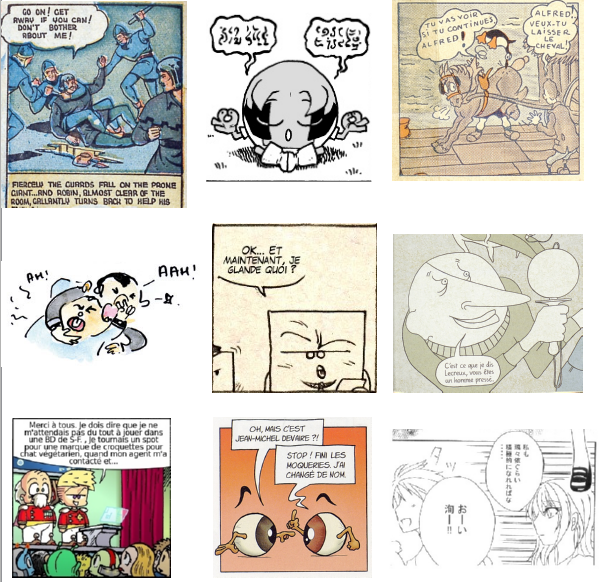
\includegraphics[trim= 4px 0px 0px 0px, clip, width=0.5\textwidth]{comics_diversity.png}
  \caption{Examples of comic panels that reflect the diversity of comics.}
  \label{fig:kn:comics_diversity}
 \end{figure}

%%%%%%%%%%%%%%%%%%%%%%%%%%%%%%%%%%%%%%%%%%%%%%%%%%

An expert system uses the ontology to assert the relations between regions and the corresponding inference engine to deduct new information in order to perform further image processing (e.g. hypotheses of the regions of interest for the localisation of comic characters or speech balloons).
Note that in the rest of the chapter ``character'' is used in the sense of actor or protagonist of the comics, not as a piece of text.
This work is the result of an extensive collaboration with Cl{\'e}ment Gu{\'e}rin, a Ph.D. student working on data mining applied to comic book contents~\cite{phdthesisGuerin14}.

%--------------------------------------------------
\section{Proposed models} % (fold)
\label{sec:proposed_models}
\subsection{Document image processing domain} % (fold)
\label{sub:document_image_processing_domain}

\paragraph{Image and regions} % (fold)
\label{par:image}
Nous avons développé dans un premier temps un modèle formalisant les notions primitives du traitement d'images.
Ce modèle se veut volontairement générique en n'intégrant aucun concept relatif à la bande dessinée afin de pouvoir être exploité dans d'autres domaines relatifs à l'analyse de documents.
Il sert de support à la structuration des données issues d'algorithmes de traitement d'images en vue de leur enrichissement sémantique ultérieur.
Les données produites par de tels algorithmes se réduisent généralement à des données spatiales, des lignes, des régions, auxquelles nous ferons indifféremment référence sous les notions de \textit{régions d'intérêt} ou \textit{ROI} (pour Region Of Interest) dans la suite de ce document.
Elle sont définies par leurs coordonnées cartésiennes dans le repère orthonormé de l'image desquelles elles sont extraites. En partant de cette vision à gros grains de ce qu'est le traitement d'image, nous définisson les deux premiers concepts de notre modèle : \concept{Image} et \concept{ROI}.\\

Le concept d'\concept{Image} modélise la notion d'image en tant qu'objet numérique, en tant que matière première du système de traitement d'images.
C'est le concept le plus général à partir duquel seront dérivés les autres concepts de notre modèle.
Un algorithme de traitement d'images fonctionne en manipulant directement les pixels de l'image, ses composants élémentaires.
Il peut les analyser indépendamment les uns des autres ou bien les regrouper par ensembles mais au final, la valeur, l'intensité de chaque pixel a son importance dans le processus d'analyse et peut avoir des conséquences sur les résultats de sortie.
Or, pour deux images d'apparence similaire aux yeux d'un observateur humain, la valeur individuelle de chacun de leurs pixels peut grandement varier d'une image à l'autre.
Elles peuvent avoir une définition différente, c'est à dire des dimensions (mesurées en pixels) différentes.
Dans le cas d'images numérisées, si les documents d'origine étaient de même taille, cette différence de définition est la conséquence d'une différence de résolution de numérisation.
La résolution d'une image indique le nombre de pixels utilisés pour discrétiser un pouce de l'espace.
Plus la résolution est élevée, plus l'image est nette.
De plus, l'encodage de l'information visuelle au sein de chaque pixel varie également en fonction du format d'image utilisé et du degré de compression avec ou sans pertes appliqué.
Il est important d'intégrer au modèle ces informations à propos de chaque image car elles sont le contexte de travail dans lequel se place l'outil d'analyse.
Elles conditionnent et permettent d'interpréter et de comprendre la qualité des résultats produits.


Le concept \concept{ROI} est un méronyme du concept \concept{Image}, c'est à dire qu'une région d'intérêt est une portion d'image, qu'elle fait partie d'une image.
Ce concept formalise la notion de région d'intérêt telle qu'elle est perçue par l'analyste d'images, c'est à dire une surface finie incluse dans le plan de l'image, composée de pixels connexes possédant des caractéristiques visuelles correspondant à une certaine classe d'objets visuels recherchés.
Le fait qu'une région d'intérêt soit une surface en deux dimensions, finie et fermée, nous permet de la représenter sous la forme d'un polygone.\\

\modif{TODO: English version}
The image model is mostly composed of the concepts of \textit{Image}, \textit{Region of interest (ROI)} and \textit{Extractor}.
It is based on the fact that the output of image analysis algorithms usually corresponds to spatial regions within the image context.
A ROI is necessarily extracted from one and only one image, and by one and only one extractor.
Therefore, the ROI concept is linked to the \textit{Image} and \textit{Extractor} concepts respectively with functional properties \textit{hasImage} and \textit{hasExtractor}.
%Their coordinates are stored in the OpenGIS Well-Know Text (WKT) format \cite{OpenGISConsortiumInc.2011}.

Algorithms may have specific characteristics so they don't produce the same set of regions as the result of the analysis of an image.
Extractors are also usually designed to extract one kind of elements (e.g. panels, balloons and text).
The purpose of each algorithm is given through the data property \textit{roiType}.
Figure~\ref{fig:kn:model_image} shows a visual representation of these concepts altogether.

 \begin{figure}[!ht]
   \centering
  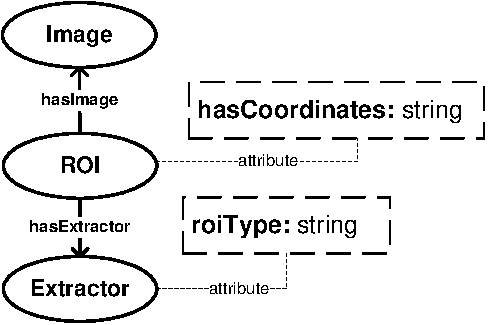
\includegraphics[width=0.5\textwidth]{model_image.pdf}
  \caption[A representation of the image model involved in the expert system]{A representation of the image model involved in the expert system. Concepts are represented by the oval-shaped items, the arrows are the object properties linking them to each other. The dashed rectangles contain the data properties of the concepts they are attached to.}
  \label{fig:kn:model_image}
 \end{figure}

%Moreover, they can be automatic but they also can be manual, if we consider a manual ground truth as a kind of extractor.
%The concept of extractor is extended in two subsumed concepts, \textit{Algorithm} and \textit{GroundTruth}.
%The resulting regions of interest of instances of one of these extractors, are respectively classified as \textit{Automatic regions (ROI\_Auto)} and \textit{Ground truth regions (ROI\_GT)}.

% paragraph image (end)

\paragraph{Region extractors} % (fold)
\label{par:region_extractor}
Le traitement d'images, et particulièrement la reconnaissance de formes, est une discipline complexe.
L'algorithme générique permettant d'identifier n'importe quel type de forme, n'importe quel objet dans une image, qu'elle représente une scène naturelle, un document ou qu'elle ait été générée numériquement, n'existe pas.
En fonction de la tâche qu'il cherche à accomplir, du type de contenu qu'il souhaite détecter, voire reconnaitre, dans une image, le chercheur met en place des techniques adaptées aux caractéristiques visuelles de ce contenu.
Il va par exemple tantôt se concentrer sur la texture, tantôt sur la couleur selon qu'il souhaite identifier des formes aux motifs connus et répétitifs, comme la surface de la mer ou le pantalon blanc et bleu d'Obélix, ou identifiables par une teinte donnée, comme par exemple un ciel bleu ou le pantalon rouge d'Astérix.
La forme de ces éléments, leur taille, leur position absolue ou relative ou encore leur orientation sont autant d'éléments parmi bien d'autres permettant de façonner un outil adapté à la tâche à accomplir.\\

Un algorithme de traitement d'images a donc généralement pour fonction la détection d'un seul type d'objet.
Toutefois, si son domaine de compétence est limité, il est souhaitable que cet algorithme soit assez robuste pour produire des résultats corrects sur un grand nombre d'images différentes.
Dès lors, le chercheur souhaitant analyser un ensemble de documents complexes mais de même nature, dans le sens où ceux-ci sont composés d'un ensemble d'éléments graphiques différents mais toutefois commun au corpus de documents, va devoir mettre en place autant de traitements spécifiques que de types d'éléments qu'il souhaite extraire, tout en prenant garde à ce qu'ils fonctionnent sur le plus grand nombre de documents possible.\\

Si nous nous plaçons par exemple dans le cadre d'un traitement automatique de documents administratifs, tels que des fiches de paye ou des factures, il pourrait être intéressant de mettre en place des systèmes permettant de détecter les logos, les caractères alphanumériques ou encore les signatures.
Si nous nous replaçons dans le contexte de la bande dessinée, la segmentation des cases, des bulles, du texte et des personnages, nécessite autant d'algorithmes d'analyse d'images différents, comme nous avons pu le voir en \ref{sec:sota_image}.
Chaque algorithme va tirer parti de ce qui fait la spécificité des éléments à extraire.
Les cases sont des éléments majeurs de l'image en terme d'espace occupé dans la page. 
Elles sont généralement délimitées par une bordure noire et séparées les unes des autres par une gouttière.
Leur forme, souvent rectangulaire, la plupart du temps au moins polygonale est également un critère utilisé, notamment via la détection des lignes dans l'image.
Les bulles contiennent du texte, traditionnellement de couleur foncée sur un fond clair.
Elles sont également délimitées par un contour noir mais ont généralement des dimensions inférieures à celles de cases.
Les lignes de texte sont composées de petits éléments visuels, contrastant avec le fond de l'image, ponctuellement alignés de manière régulière.
Des techniques de reconnaissance de caractères (OCR) peuvent éventuellement venir en renfort afin de filtrer les faux-positifs.
Les personnages de bande dessinée peuvent avoir n'importe quelle forme, réaliste ou caricaturale, humanoïde ou non.
Ils présentent en revanche une certaine régularité dans leur représentation visuelle.
Ils peuvent changer de position, d'orientation ou de dimensions mais ils conservent la plupart du temps les mêmes attributs vestimentaires, les mêmes caractéristiques visuelles, au moins le long d'une même histoire.\\

%\modif{Serait-ce intéressant de rentrer un petit plus en détails dans les techniques d'analyse d'images de bande dessinée ? Intégrer quelques références ?}\\

Une région d'intérêt identifiée par un algorithme de segmentation d'images correspond donc à la proposition par ce dernier d'une zone spatiale de l'image contenant le type d'élément qu'il a été conçu pour détecter.
Cette région peut effectivement contenir un élément de ce type ou bien contenir tout autre chose.
La précision de segmentation de l'algorithme est dépendante à la fois des caractéristiques de l'image analysée, de la complexité du domaine d'analyse et bien sûr de la qualité de son implémentation.
L'ensemble des résultats peut contenir des erreurs.
Les régions d'intérêt produites ne sont que des propositions demandant à être vérifiées, elles n'ont pas valeur de vérité.\\

Nous appellerons de tels systèmes de segmentation \textit{extracteurs} dans la suite de ce document.
La notion d'extracteur est intégrée dans notre modèle sous le concept \concept{Extractor}.
Relié à celui de \concept{ROI}, il permet d'exprimer le lien étroit entre l'algorithme de traitement d'images et les régions d'intérêt qu'il produit à partir d'une image aux caractéristiques données.
%de modéliser la connaissance liée aux spécificités d'un extracteur et des régions d'intérêt qu'il produit par rapport à une image aux caractéristiques données.
Cet ensemble de notions fournit un premier cadre à l'évaluation de la pertinence de l'intégration d'une ROI dans un système plus complet où elle sera amenée à interagir avec d'autres entités.
Une région d'intérêt provenant d'une image est produite par un et un seul extracteur.
% paragraph paragraph_name (end)

% subsection document_image_processing (end)
\subsection{Comics domain} % (fold)
\label{sub:comics_domain}
Nous présentons dans cette section une conceptualisation du domaine de la bande dessinée ainsi que sa formalisation ontologique.
Cette conceptualisation a été pensée en gardant à l'esprit l'objectif d'une utilisation dans le cadre de l'analyse d'images.
Des amendements y seront apposés plus tard dans ce manuscrit afin de rendre son utilisation possible dans d'autres cadres applicatifs.

\paragraph{Album and pages} % (fold)
\label{par:album_and_pages}
Comme nous l'avons vu dans le chapitre~\ref{chap:codes_bd}, une bande dessinée se définie comme une suite d'images transmettant un message.
Ces images sont spatialement juxtaposées dans un plan que l'on nomme \emph{planche}.
Dans la bande dessinée que l'on peut qualifier de classique, franco-belge, américaine et japonaise, une histoire se raconte à travers une succession ordonnée de planches.
Celles-ci sont matérialisées par des pages imprimées regroupées au sein d'un album, ce dernier pouvant lui même n'être qu'une itération d'une collection contant une histoire plus large.
Les webcomics font également usage de planches, matérialisées par des images numériques.
Dans le cas de la bande dessinée imprimée, une planche peut s'étendre sur une ou deux pages, rarement plus.
Une planche de webcomic est toujours représentée par une image unique.


Les deux premiers concepts introduits sont alors \textit{Comic} et \textit{Plate}\footnote{Le vocabulaire français possède une distinction claire entre les termes planche et page. Les anglophones ont cependant tendance à utiliser le mot \emph{page} pour désigner ces deux notions. Le terme \emph{plate}, moins usité, a été sélectionné afin de désambiguïser ces deux notions.}, représentant respectivement les notions d'album et de planche.
Ces deux concepts sont liés par la propriété \textit{hasPlate}.
Celle-ci est inversement fonctionnelle, une planche ne pouvant faire partie que d'un seul album.

Les informations bibliographiques de chaque album sont représentées par des attributs associés au concept \concept{Comic}.
Le titre de l'album, l'éventuelle collection de laquelle il est issu, ses auteurs, sa date de publication ou encore son ISBN peuvent être renseignés via les attributs correspondants.
La direction de lecture (de gauche à droite ou de droite à gauche) peut être indiquée à travers l'attribut booléen \dataProp{right2Left}.


% paragraph album_and_pages (end)

\paragraph{Page content} % (fold)
\label{par:page_content}
Comme présenté dans le chapitre~\ref{chap:codes_bd}, une planche de bande dessinée est le cadre dans lequel sont placées les cases constituant le récit.
L'ordre de ces cases dans la séquence de lecture est défini par leur position relative les unes par rapport aux autres ainsi que, dans certains cas, l'interprétation personnelle du lecteur.
L'étude et la génération de la séquence de lecture est l'objet de la section~\ref{sec:ordre}.
Le contenu des cases est composé de dessins représentant notamment des personnages et des phylactères.
Nous avons choisi de nous concentrer sur les relations entre ces deux types de contenu dans un premier temps.
La gestion des autres éléments représentés au sein des cases dépasse le cadre de ces travaux, bien qu'une approche basée sur une extraction de termes appropriés depuis WordNet, similaire à celle proposée par \cite{Zinger2005}, pourrait se révéler intéressante.
Les phylactères contiennent eux-même des lignes de texte, matérialisant les mots des personnages et la narration de l'histoire.\\

%le contenu d'une planche est principalement composé de cases, de phylactères et de texte.
%Les différents plans ponctuant l'histoire sont dessinés à l'intérieur des cases.
%Ils mettent notamment en scène les personnages prenant part au récit.

Les cases sont représentées par le concept \concept{Panel}.
Celui-ci possède pour un attribut \dataProp{hasRank} indiquant la place de chacune de ses instances dans la séquence de lecture de la planche à laquelle elles sont rattachées.

Les phylactères, qu'il s'agisse de bulles de dialogue, de pensée ou de cadres de narration, sont représentés par le concept \concept{Balloon}.
D'une manière similaire aux cases dans la planche, les bulles doivent être lues selon un ordre défini par leur position dans leur case de rattachement.
On parle de case de \emph{rattachement} et non pas de case \emph{englobante} car, selon les styles de bandes dessinées, les bulles se sont pas nécessairement positionnées spatialement à l'intérieur d'une case.
Il arrive qu'elles soient légèrement à l'extérieur ou à cheval sur plusieurs cases.
En revanche, chaque case met en images une action se déroulant à un instant fixe.
Les bulles font partie intégrante de la mise en scène et sont donc rattachées à une case donnée, quelle que soit leur position par rapport à cette case.
Leur place dans l'ordre de lecture d'une case est défini par l'attribut \dataProp{hasRank} et la propriété \objProp{hasNextBalloon} lie les bulles entre elles.

Les bulles de dialogue possèdent une ou plusieurs excroissances sur leur contour, appelées flèches ou queues, pointant vers le ou les personnages dont elles matérialisent les paroles.
Cette flèche est représentée par le concept \concept{Tail}, et sa direction par l'attribut \dataProp{hasDirection}.
Une bulle est liée à une ou plusieurs flèches par la propriété \objProp{hasTail}.


Les lignes de texte sont représentées par le concept \concept{TextLine}.
Elles sont regroupées à l'intérieur de phylactères et se lisent naturellement de haut en bas.
Comme pour les cases et les bulles, l'attribut \dataProp{hasRank} permet de spécifier leur place dans la séquence de lecture au sein d'une bulle, la propriété \objProp{hasNextTextLine}.
Le texte de la ligne est retranscrit par l'attribut \dataProp{hasText}.


Les concepts \concept{Panel}, \concept{Balloon}, 
\concept{Tail}, 
\concept{TextLine} et \concept{Character} sont disjoints, un élément ne pouvant être instance que de l'un d'entre eux.\\

La figure~\ref{fig:model_d_2} illustre l'ajout de ces concepts à notre ontologie.\\

\begin{figure}[h!]
\begin{center}
%\includegraphics[width=1\textwidth]{img/contributions_domaine/model_step2.pdf}
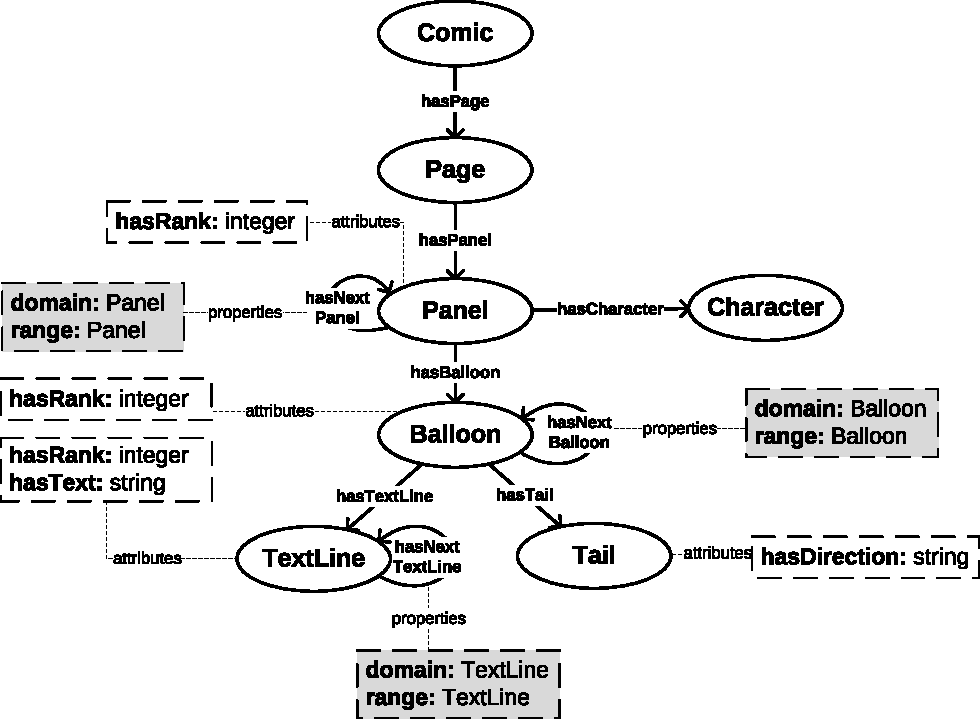
\includegraphics[width=1\textwidth]{model_step2_new.pdf}
\caption[Ontologie bande dessinée - Deuxième étape]{Modèle présenté en figure~\ref{fig:model_d_1} enrichi des concepts \concept{Panel}, \concept{Balloon}, \concept{TextLine} et \concept{Character}.}
\label{fig:model_d_2}
\end{center}
\end{figure}

Plusieurs propriétés sont introduites dans notre ontologie afin de représenter les liens existants entre les différents éléments composant une planche.
Une case étant relative à une planche, la propriété \objProp{hasPanel} lie une instance de \concept{Plate} à une instance de \concept{Panel}
Le domain et le range de la propriété assurent que seule une planche et une case puisse en être respectivement le sujet et l'objet.
La propriété \objProp{hasPanel} est également définie inversement fonctionnelle, une case ne pouvant faire partie que d'une seule planche.

Les propriétés \objProp{hasBalloon} et \objProp{hasCharacter} sont définies formellement de manière similaire et représentent le lien d'appartenance existant entre, d'une part, une case et, d'autre part, une instance de \concept{Balloon} et de \concept{Character}.
La propriété \objProp{hasTextLine} représentent l'appartenance d'une ligne de texte à un phylactère.
Nous avons ici opté pour une conceptualisation très contrainte mettant de côté certains cas de figure non négligeables, notamment celui des lignes de texte hors phylactères.
Cela se justifie dans le cadre d'une analyse automatique d'images, comme nous le présentons au chapitre~\ref{chap:analyseImage}.\\

Une certaine transitivité dans l'inclusion des éléments les uns par rapport aux autres est observable.
Les lignes font partie des bulles, faisant elles mêmes, tout comme les personnages, parties des cases.
Les cases sont regroupées au sein de planches qui, mises les unes à la suite des autres, forment un album.
L'exploitation de ces appartenances successives trouve un intérêt certain dans un contexte de recherche d'informations au sein d'une base de connaissances.
Une requête portant sur les albums où apparaissent dans une même case plusieurs personnages prononçant certains termes pourrait par exemple s'affranchir des notions de planche et de bulle.
% paragraph page_content (end)

\paragraph{Specialization of the content} % (fold)
\label{par:specialization_of_the_content}

La sémantique de certains concepts reste d'un degré de granularité assez grossier avec la conceptualisation présentée jusqu'à présent.
Les phylactères peuvent notamment se catégoriser en deux sous-ensembles.
D'un côté les bulles émises par des personnages (à voix haute ou pensées) ou des éléments de la scène (radio, télévision, etc.), d'un autre coté les cadres de narration.
La forme des phylactères varie d'un auteur ou d'une époque à l'autre.
Un élément semble faire consensus pour discriminer les bulles des encadrés, c'est la présence, ou non, d'une queue pointant vers la source du son.\\

Les concepts \concept{NarrativeBalloon} et \concept{SpeechBalloon} sont introduits afin de représenter respectivement les phylactères dont le contenu fait progresser la narration d'une manière ou d'une autre (encadrés, dialogue, etc.), et les bulles matérialisant spécifiquement une section de discours, qu'il soit pensé ou récité à voix haute.
Ces éléments sont caractérisés par la présence de lignes de texte, les bulles de discours étant en plus équipées d'une flèche pointant vers la source du son.
Ils sont définis par les formules~\ref{eq:narrativeBalloon} et \ref{eq:speechBalloon}.

La sémantique des lignes de texte appartenant à ces nouvelles classes de phylactères peut alors également être affinée en conséquence.
Certaines lignes sont porteuses d'éléments de discours, tandis que d'autres sont, d'une manière plus générale, au service de la narration.
Les concepts introduits pour représenter ces deux notions sont \concept{SpokenTextLine} et \concept{NarrativeTextLine}.
Ils simplement définis comme des lignes de texte appartenant respectivement à une instance de \concept{SpeechBalloon} ou de \concept{NarrativeBalloon}.


Les bulles de dialogue sont généralement émises par un personnage présent dans la case.
Le lien entre un personnage et une bulle de dialogue est exprimé à travers la propriété \objProp{says}, ayant pour domain \concept{Character} et pour range \concept{SpeechBalloon}.
Le concept \concept{Speaker} représente les personnages émettant des bulles de dialogue.


La figure~\ref{fig:model_d_3} illustre les relations de subsomption introduites sur les concepts \concept{Balloon}, \concept{TextLine} et \concept{Character}.\\

\begin{figure}[h!]
\begin{center}
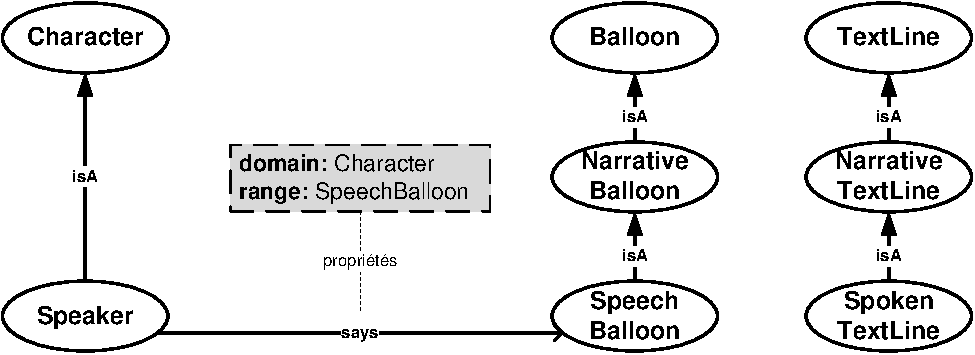
\includegraphics[width=1\textwidth]{model_step2ter_new.pdf}
\caption{Spécialisation des concepts \concept{Character}, \concept{Balloon} et \concept{TextLine}}
\label{fig:model_d_3}
\end{center}
\end{figure}

\modif{TODO: English version}

Semantic relations were also defined in order to categorise some region types such as balloons into speech balloon $SB$ (versus narrative balloons), characters into speaking characters $SC$ (versus non-speaking characters) and text lines as speech text $ST$ (versus narrative lines):
\begin{itemize}
  \item A $SB$ is a balloon $B$ that has a tail and contains text
  \item A $SC$ is a character $C$ pointed by a tail
  \item A $ST$ is a text line which is included in one speech balloon
\end{itemize}

The term ``pointed'' refers to the fact that the character is included in the part of the panel indicated by the tail. To have a better understanding of how a panel is divided according to tail direction, please refer to Section~\ref{sec:se:tail_to_character}.

These figures represent the theoretical limit that can be reached with the model in terms of component extraction performance.
% section knowledge_representation (end)

% paragraph specialization_of_the_content (end)

\modif{TODO: English version}
The first level of our comics model taxonomy is composed of the concepts of \textit{Album}, \textit{Pages} and \textit{Content}.
\textit{Album} is linked to \textit{Page} and \textit{Page} to \textit{Content} respectively by the \textit{hasPage} and \textit{hasContent} properties.
The concept of \textit{Content} stands for any kind of visual element that can appear on an analysed page of comic book.
It is specialized into the concepts of \textit{Panel}, \textit{Balloon}, \textit{TextLine} and \textit{Character}.
As it was stated in Section~\ref{sec:kn:constrains_low_level_extraction}, we consider that panels are only contained by a page, characters and balloons by panels and lines of text by balloons.
This is modelled with object properties with constrained domain and range.
The \textit{hasPanel}, \textit{hasBalloon}, \textit{hasTextLine} and \textit{hasCharacter} properties link a page to a panel, a panel to a balloon, a balloon to a line and a panel to a character, respectively.

Even if that does not cover every situation (text lines can sometimes be found outside of balloons, e.g onomatopoeia), these constrained properties are necessary to use these models as validation tools.
%While we know that it does not cover every different kind of comics material, it is necessary if we want it constrained enough to be usable as a segmentation validation tool.
The concepts of \textit{Speaker}, \textit{SpeechBalloon} and \textit{SpokenTextLine} are subsumed by \textit{Character}, \textit{Balloon} and \textit{TextLine} respectively and are derived with an OWL translation of the rules defined Section~\ref{sec:kn:constrains_low_level_extraction}.
This hierarchy is visually represented in Figure~\ref{fig:kn:model_image}.
Balloons and text lines are also enriched by some attributes, like the direction indicated by the tail (\textit{tailDirection}) or the textual transcription of the text lines (\textit{hasText}).

 \begin{figure}[!ht]
   \centering
  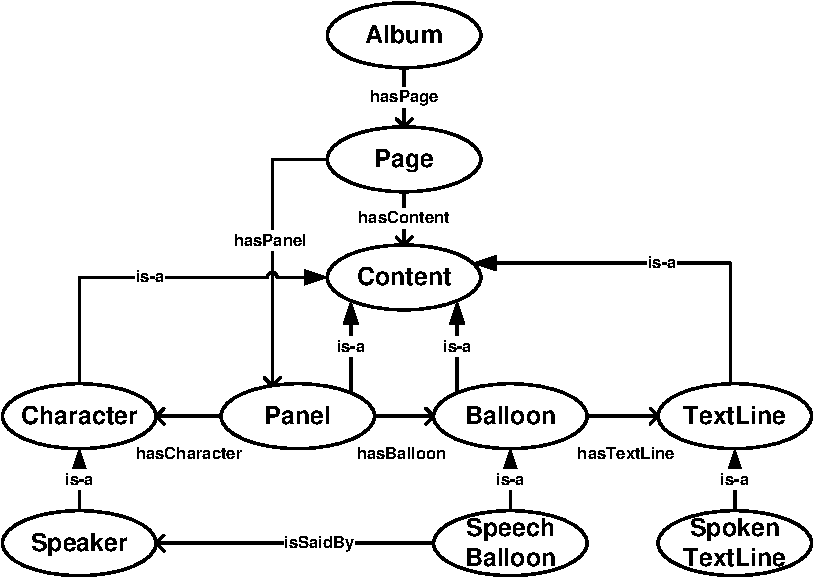
\includegraphics[width=0.7\textwidth]{model_comics.pdf}
  \caption[A representation of the main aspects of the comics model involved in the expert system]{A representation of the main aspects of the comics model involved in the expert system. Concepts are represented by the oval-shaped items, full arrows represent subsumption relations, simple arrows are the object properties linking them to each others. Attributes are not displayed to make it more comprehensible.}
  \label{fig:kn:model_image}
 \end{figure}

% subsection comics_domain (end)

\subsection{Model interactions} % (fold)
\label{sub:model_interactions}

\modif{
  
Nous allons voir dans cette section comment connecter l'ontologie image, notée ici $\mathcal{O}_{image}$, et l'ontologie de la bande dessinée, $\mathcal{O}_{bd}$, des sections~\ref{sec:modele_image} et \ref{sec:modele_domaine} afin qu'elles puissent communiquer et que leurs capacités de raisonnement respectives puissent être exploitées.
Ces deux modèles ont été développés en vue d'être utilisés dans un système d'analyse d'images de bandes dessinées.
Dans ce contexte, nous considérons que l'image numérisée d'une planche est la matière première fournie à un algorithme pour qu'il puisse extraire son contenu.


Comme cela a été souligné précédemment, un algorithme d'analyse d'images a pour objectif la détection de caractéristiques visuelles discriminant un type d'objet particulier.
Dans notre cas, les extracteurs développés concernent les cases, les bulles, 
la queue des bulles, 
le texte et les personnages.

La figure~\ref{fig:interaction} illustre ces interactions entre les ontologies.\\

}


\begin{figure}[h!]
\begin{center}
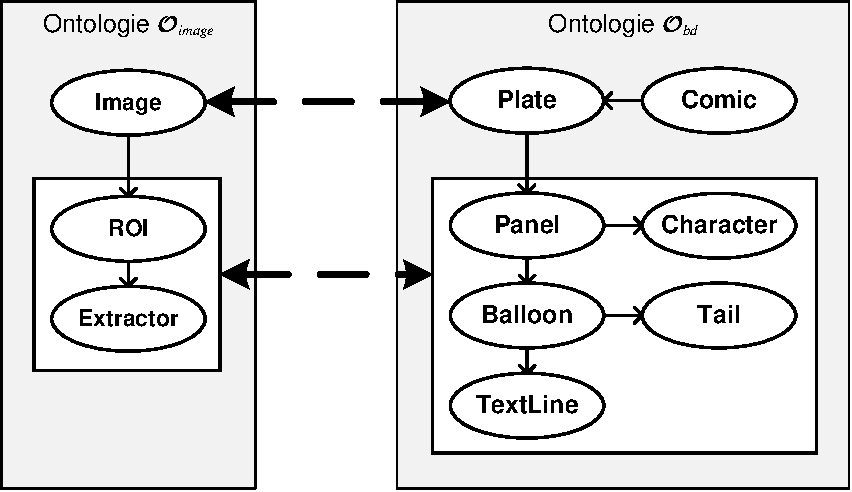
\includegraphics[width=0.8\textwidth]{interaction.pdf}
\caption{Interaction entre les ontologies image et bande dessinée}
\label{fig:interaction}
\end{center}
\end{figure}

The image and comics models are linked through two bridges.
First, the \textit{Image} from the image model and \textit{Page} from the comics model concepts are made equivalent by the axiom \texttt{owl:equivalentClass}.
This way we ensure that all extracted content related to an image is equally related to a corresponding page in the comics domain $Page \equiv  Image$.

Second, the classes $Cl=\{Panel$, $Balloon$, $TextLine$, $Character\}$ are defined as equivalent to the corresponding set of regions of interest $Sr = \{panels$, $balloons$, $text lines$, $characters\}$ Equation~\ref{eq:kn:class_region_equivalence}).% that have an extractor which purpose is to extract the corresponding panels (resp. balloons, text lines and characters).
  

\begin{equation}
\label{eq:kn:class_region_equivalence}
\begin{split}
Cl_i  \equiv \text{ROI} \textbf{ and } (hasExtractor \textbf{ some } (roiType \textbf{ value } Sr_i ))
\end{split}
\end{equation}

% subsection model_interactions (end)

% section proposed_models (end)

%--------------------------------------------------
\section{Expert system for contextual analysis} % (fold)
\label{sec:kn:expert_system}

\modif{Une dynamique de bouclage et de communication est entretenue entre les deux parties du système global d'analyse.
Il est fait référence à la partie algorithmique de traitement d'images sous le nom de \emph{système bas niveau}, sous entendu proche des données pixellaires.
Le système formé des ontologies développées, couplées à un moteur d'inférence, est dénommé ci-après \emph{système expert} pour plus de clarté.
}
The purpose of the expert system is to interact with the low level (image processing) iteratively to progressively understand the content of an image, moving from simple to more complex elements.
This approach is similar to~\cite{Sciascio2011Structured} except that in our case the definition of the complex object is not a composition of simple objects but context-driven.


\subsection{Interactions between low and high level processing} % (fold)
\label{sub:interactions_between_low_and_high_level_processing}


Nous considérons ici les ontologies $\mathcal{O}_{image}$ et $\mathcal{O}_{bd}$ développées comme parties intégrantes d'un système expert fournissant un cadre d'interprétation au contenu extrait par un système de traitement d'images bas niveau.
Le but du système expert est d'interagir de manière itérative avec le système bas niveau pour comprendre progressivement le contenu d'une page, de ses éléments les plus simples aux éléments plus complexes.
L'ensemble du système expert, représenté par le schéma de la figure~\ref{fig:expertSystem}, inclus donc les deux ontologies présentées dans le chapitre~\ref{chap:ontologies}, formant ensemble notre base de connaissances.
Cette base, une fois peuplée par des données en provenance du système bas niveau, est traitée par un moteur d'inférence pour en extraire des conclusions logiques, dépendantes des données et de leur cohérence par rapport à la connaissance formalisée.

Ces conclusions peuvent consister en la validation d'éléments extraits, en leur rejet ou la création d'individus renvoyés au système d'extraction d'images.\\

\begin{figure}[h!]
\begin{center}
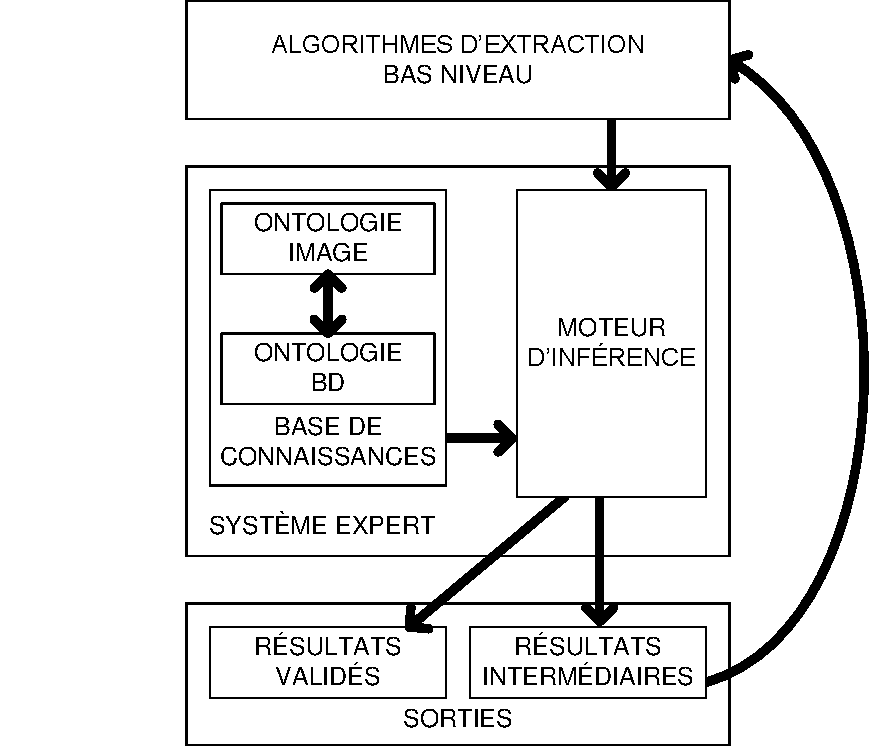
\includegraphics[width=0.85\textwidth]{expert_system_v2.pdf}
\caption[Représentation du système d'analyse]{Représentation des interactions entre les systèmes bas et haut niveau}
\label{fig:expertSystem}
\end{center}
\end{figure}

Les algorithmes bas niveau ont été développés pour extraire des éléments spécifiques depuis l'image entière d'une planche ou une région de celle-ci.
Les systèmes haut et bas niveau interagissent afin que la totalité des extractions et leurs relations soient en concordance avec la représentation de la connaissance du domaine étudié.
La figure~\ref{fig:kn:process_loop} illustre la boucle de traitement liant les deux systèmes.

A l'étape 1, le système bas niveau propose au système expert des hypothèses tenant en un premier ensemble de régions segmentées dans l'image.
Ces régions sont labellisées selon leur type supposé (cases, bulles, etc.).
Lors de la deuxième étape, le système expert évalue ces hypothèses, valide celles qu'il juge correctes et supprime celles qu'il considère erronées.
A la troisième étape, de nouvelles informations sont déduites à partir des hypothèses validées, mises en perspectives de la connaissance du domaine.
Celles-ci sont renvoyées au système bas niveau qui s'en sert, au cours d'une deuxième itération, pour extraire des éléments plus complexes, tels que les personnages.

----------------------------------------------------------------

In our system, the expert system includes two models, one formalizing the raw data from algorithms (\emph{Image model}) and the other modelling the domain knowledge of the comic books (\emph{Comics model}).
These two models are ontologies that work together to
%This knowledge is formalized in an ontology that 
express the relations between the primary elements of a document that can be considered as being stable through all instances of the studied domain (Figure~\ref{fig:kn:generic_expert_system}).
Thus, the expression of the constraints applied both to the elements and their relations have to be specific enough because these constraints will be considered as the reference knowledge for the detection of potential errors of the low-level extraction algorithm output.

%%%%%%%%%%%%%%%%%%%%%%%%%%%%%%%%%%%%%%%%%%%%%%%%%%%
 \begin{figure}[!ht]  %trim=l b r t  width=0.5\textwidth,
   \centering
  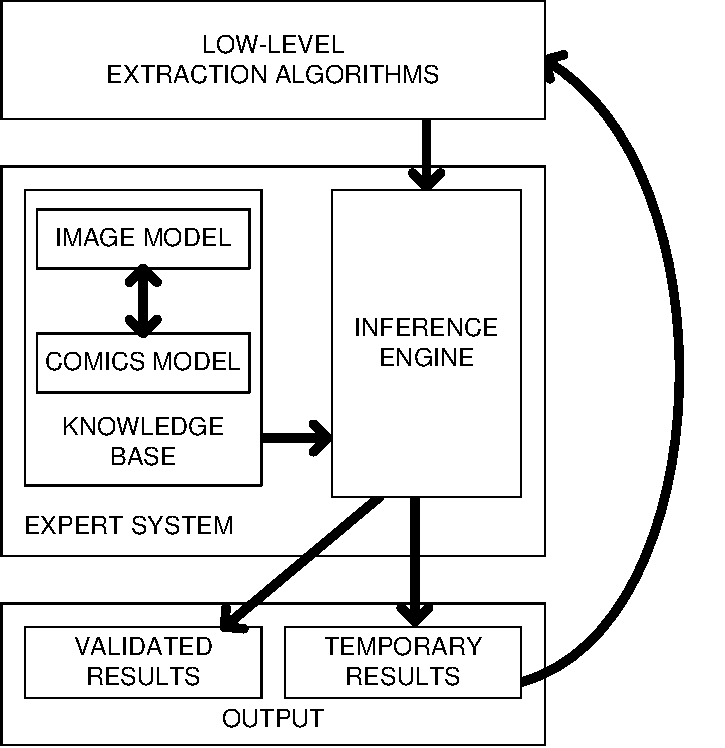
\includegraphics[trim= 0px 0px 0px 0px, clip, width=0.5\textwidth]{expert_system.pdf}
  \caption[Generic representation of the expert system and the relationship between knowledge base, the inference engine and the low-level algorithms]{Generic representation of the expert system and the relationship between knowledge base, the inference engine and the low-level algorithms.}
  \label{fig:kn:generic_expert_system}
 \end{figure}
%%%%%%%%%%%%%%%%%%%%%%%%%%%%%%%%%%%%%%%%%%%%%%%%%%%


%This knowledge can be represented by all the relations betweens the elements that constitute a document from this collection.
The low level algorithms are designed to extract specific information from the whole image or a specific region.
Low and high level systems interact in a loop to feed the knowledge base until there is a complete and consistent understanding of the document, according to the knowledge domain. 
% This loop can be summarized as follows:


%%%%%%%%%%%%%%%%%%%%%%%%%%%%%%%%%%%%%%%%%%%%%%%%%%%
 \begin{figure}[!ht]  %trim=l b r t  width=0.5\textwidth,
   \centering
  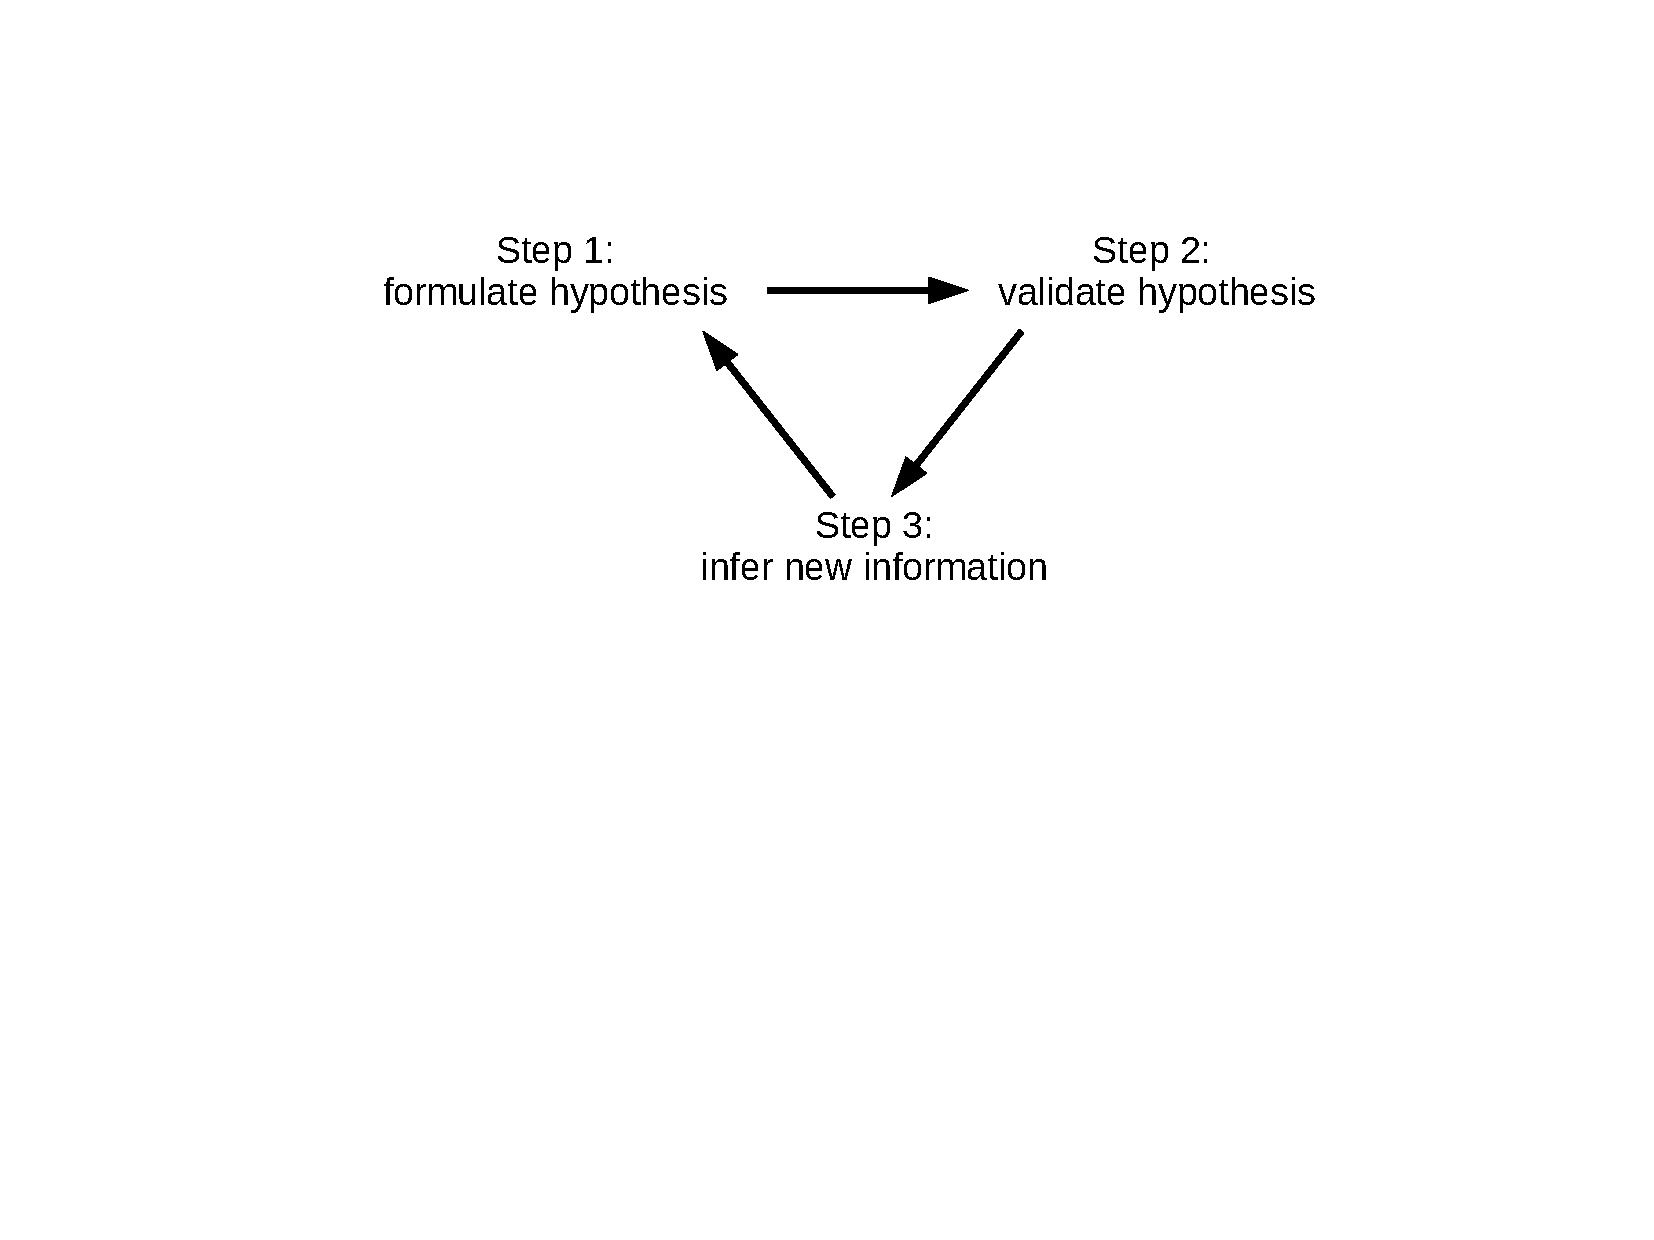
\includegraphics[trim= 140px 350px 100px 95px, clip, width=0.7\textwidth]{process_loop.pdf}
  \caption[Process loop of the knowledge-driven system]{Process loop of the framework.}
  \label{fig:kn:process_loop}
 \end{figure}
%%%%%%%%%%%%%%%%%%%%%%%%%%%%%%%%%%%%%%%%%%%%%%%%%%%

In Figure~\ref{fig:kn:process_loop}, the starting point is step 1 (formulate hypothesis) where low level processing give basic information to the expert system (populating).
%, preferably with a high recall.
Then, step 2 (validate hypothesis) assesses the valid elements and removes obvious mistakes, and in step 3 we infer new information based on the previous information and the knowledge base.
In the next iteration of the process loop, the newly validated information can be used by low level processing (e.g. new parameters, region of interest) to extract more complex elements from the image and so on.
This loop can be run as many times as new information is discovered (until being idempotent).

% subsection interactions_between_low_and_high_level_processing (end)


% section expert_system (end)

\subsection{Constrains for the low level extractions} % (fold)
\label{sec:kn:constrains_low_level_extraction}
In our model, knowledge is modelled though the categorization of each element composing a page, combined with a set of topological relation with these elements.
In our context, the elements that compose a given image $I$ are panels $P$, balloons $B$, tails $Q$, text $T$ and characters $C$, as well as the set of topological relations between them.
Because comics, as an art form, do not follow any strict specifications it is really hard to build a perfect model which is valid for all kinds of comics.
There are some instances of comic books without balloons or without panels.
If webcomics are also considered, then a comic is not even necessarily composed of pages.
A model that would be true for every type of comic book would be too general to be of any use in this work.
Instead we define a general comic book model with more constrained properties that represent a large subset of comics (Franco-Belgian, Japanese and American).
The main advantage is that it can be adapted to any kind of document images by defining properties according to the application domain.
We define the general properties of comics as follows:

\begin{itemize}
  \item A panel $P$ is related to one and only one comics page
  \item A balloon $B$ is related to one and only one panel
  \item A character $C$ is related to one and only one panel
  % \item A same character can appear only once in a panel
  \item A text line $T$ is related to one and only one balloon $B$
\end{itemize}

Despite the fact that authors are entirely free in their layout choices, some researchers insist a few conventions, widely adopted by comic book' authors, be respected to avoid the reader being confused\cite{Laine2010,Duc1982}.
The depicted elements and their place in the layout must be clearly identifiable at first sight, meaning, for instance, that balloons and characters should be included inside panels.
Whereas one can find some instances of balloons breaking out of their frame, these are usually kept to a minimum.

Therefore, the term ``related'' refers to the situation where an object is overlapped (a fortiori, contained) by another over a \emph{significant} proportion of its surface.
% refers to the smallest region (panel, balloon or text line) covering the object on more than a predefined proportion of its size.
In the case of multiple intersections, only the smallest container is considered.
When the element is fully contained in several other items, the smallest container is consequently the direct container (e.g. a text line must be considered as being included inside a balloon before being included inside the panel containing that balloon).

\section{Processing sequence (\modif{6.3 Clement})} % (fold)
\label{sec:kn:framework_}

\modif{TODO: complete with Clement's details}

The expert system asserts the extraction of simple elements such as panels, texts, balloons and tails in order to infer speech balloons before searching for more complex elements (e.g. comic book characters) based on the context defined by the simple elements and their relations.
This can be demonstrated with the first two iterations of the process loop (Figure~\ref{fig:kn:process_loop}).
The process flow of the two iterations is detailed hereafter.

\subsection{Simple element extraction} % (fold)
\label{sub:simple_element_extraction}

\paragraph{Iteration 1 - step 1 (hypothesis)} % (fold)
\label{par:step_1}
The initial extraction of panels, text and balloons feeds the knowledge base.
All the elements are extracted independently using the method proposed Chapter~\ref{chap:independent}.
% given an hypothesis on the labels of each region according to the extractor it is from (e.g. for a region from the balloon extractor, the hypothesis is a balloon label).
In Figure~\ref{fig:kn:graph0}, dashed elements represent the initial hypotheses and each layer a result from a different extractor.
Note that extraction errors can take place at this stage which the system can recover from at a later stage.
% have been introduced in the example in order to demonstrate how the proposed system can recover them.
% The regions that have been validated by the expert system have a solid border, others a dashed border.


%%%%%%%%%%%%%%%%%%%%%%%%%%%%%%%%%%%%%%%%%%%%%%%%%%%
 \begin{figure}[!ht]  %trim=l b r t  width=0.5\textwidth,
   \centering
   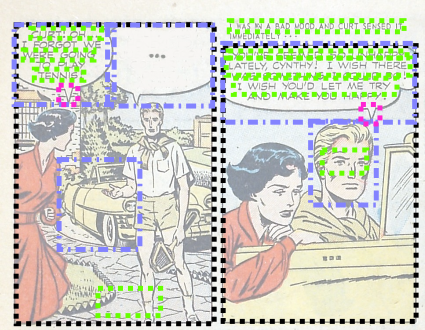
\includegraphics[trim= 0px 0px 0px 0px, clip, width=0.5\textwidth]{process_illustration_hypo_1.png}\\
  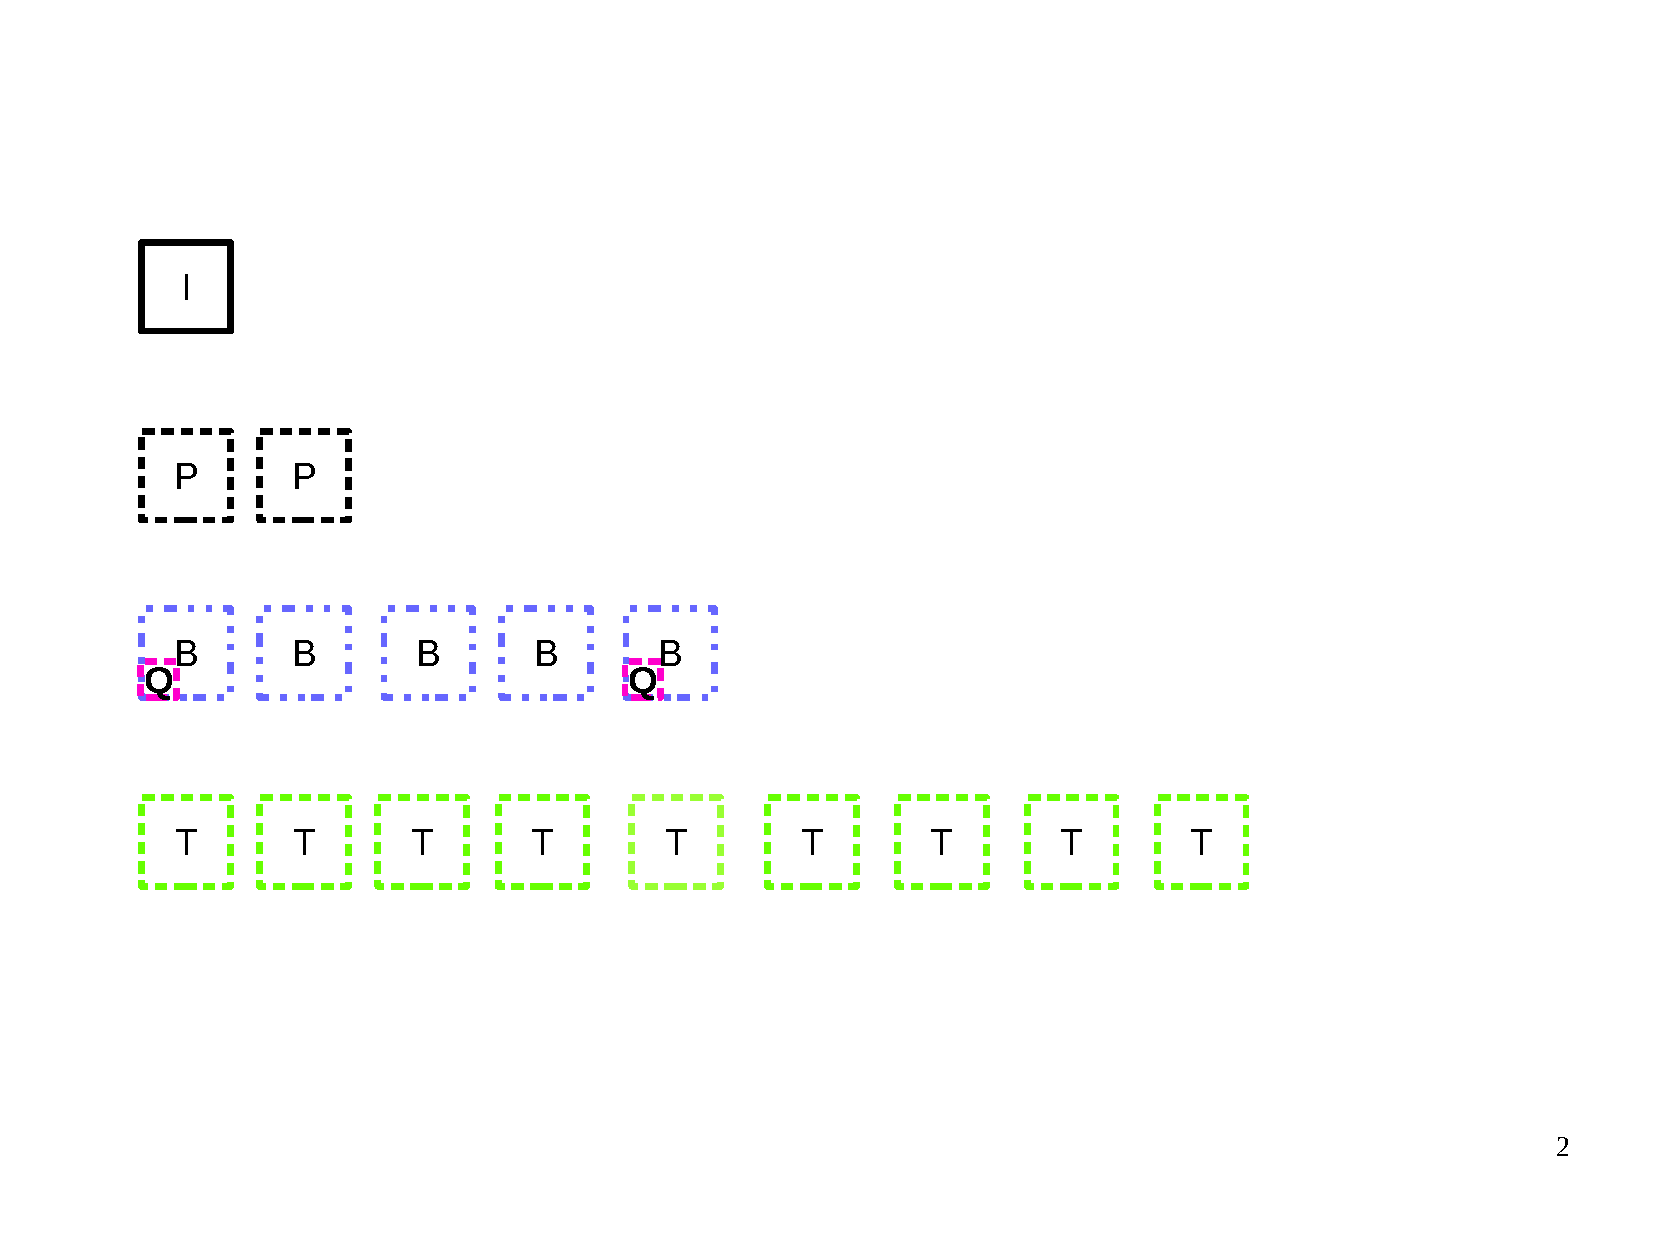
\includegraphics[trim= 30px 168px 100px 110px, clip, width=0.8\textwidth]{graph_init_1_non_orderred.pdf}
  \caption[Initial hypothesis about the content of a given image]{Initial hypothesis (dashed elements) about the content of a given image $I$ after the initial extractions of panels $P$, text $T$ and balloons $B$ with tails $Q$.
  }
  \label{fig:kn:graph0}
 \end{figure}
%%%%%%%%%%%%%%%%%%%%%%%%%%%%%%%%%%%%%%%%%%%%%%%%%%%

\paragraph{Iteration 1 - step 2 (validation)} % (fold)
\label{par:step_2}
Subsequently, the expert system checks if their spatial relations (context) match the topological properties of the knowledge base defined Section~\ref{sec:kn:constrains_low_level_extraction}, otherwise it solves them using the domain knowledge described in Section~\ref{sub:kn:validation}.
The result is illustrated in Figure~\ref{fig:kn:graph_valid_initial}.


%%%%%%%%%%%%%%%%%%%%%%%%%%%%%%%%%%%%%%%%%%%%%%%%%%%
 \begin{figure}[!ht]  %trim=l b r t  width=0.5\textwidth,
   \centering
   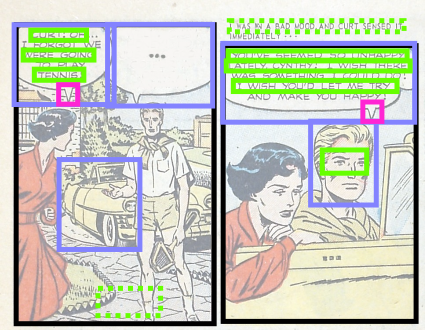
\includegraphics[trim= 0px 0px 0px 0px, clip, width=0.5\textwidth]{process_illustration_valid_1.png}\\
  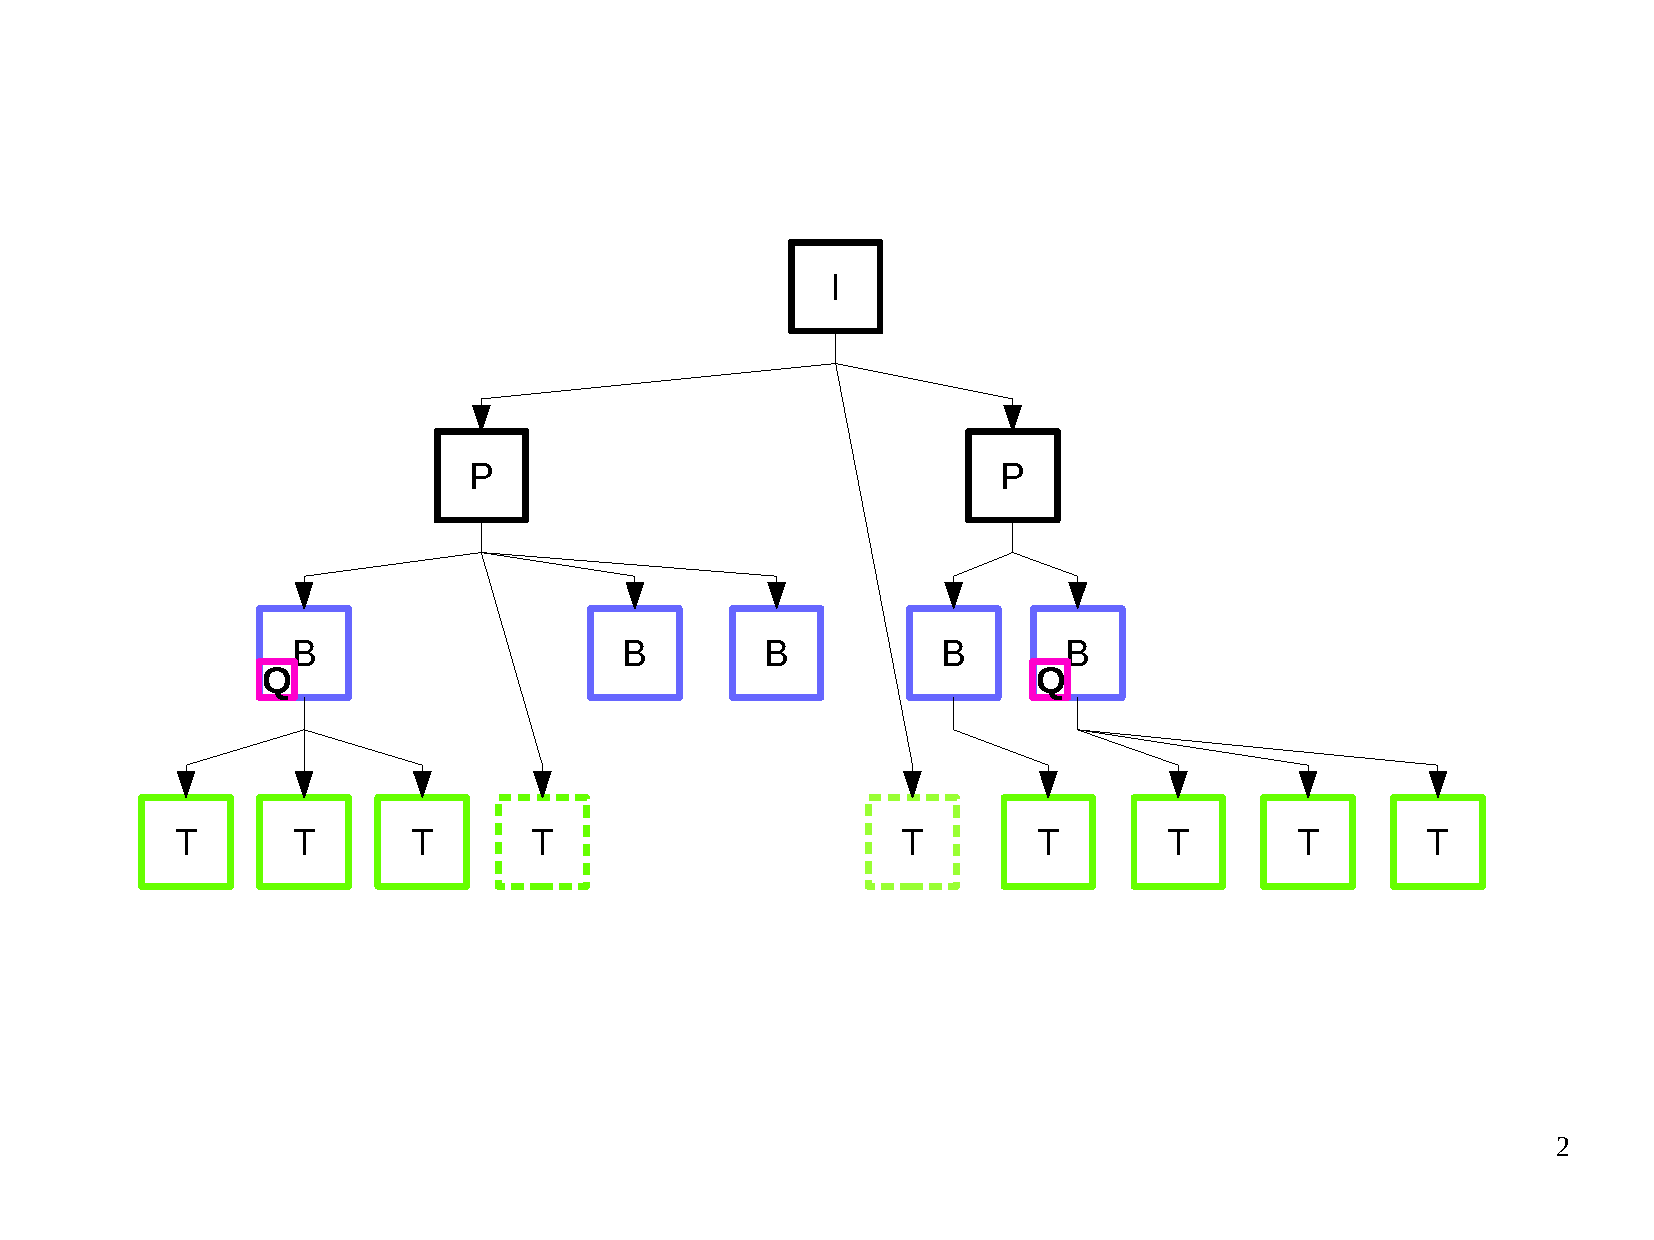
\includegraphics[trim= 30px 168px 20px 110px, clip, width=0.8\textwidth]{graph_valid_1.pdf}
  \caption[Validation of the hypothesis using the properties of the knowledge base]{Validation of the hypothesis using the properties of the knowledge base. Valid elements have a solid border.}
  \label{fig:kn:graph_valid_initial}
 \end{figure}
%%%%%%%%%%%%%%%%%%%%%%%%%%%%%%%%%%%%%%%%%%%%%%%%%%%

\paragraph{Iteration 1 - step 3 (inference)} % (fold)
\label{par:step_3}
From the validated information, the expert system infers the semantic information between text and balloon and specifies them as speech balloon and speech text respectively when they verify the properties of the knowledge base (Figure~\ref{fig:kn:graph_specific_types}). 

%%%%%%%%%%%%%%%%%%%%%%%%%%%%%%%%%%%%%%%%%%%%%%%%%%%
 \begin{figure}[!ht]  %trim=l b r t  width=0.5\textwidth,
   \centering
  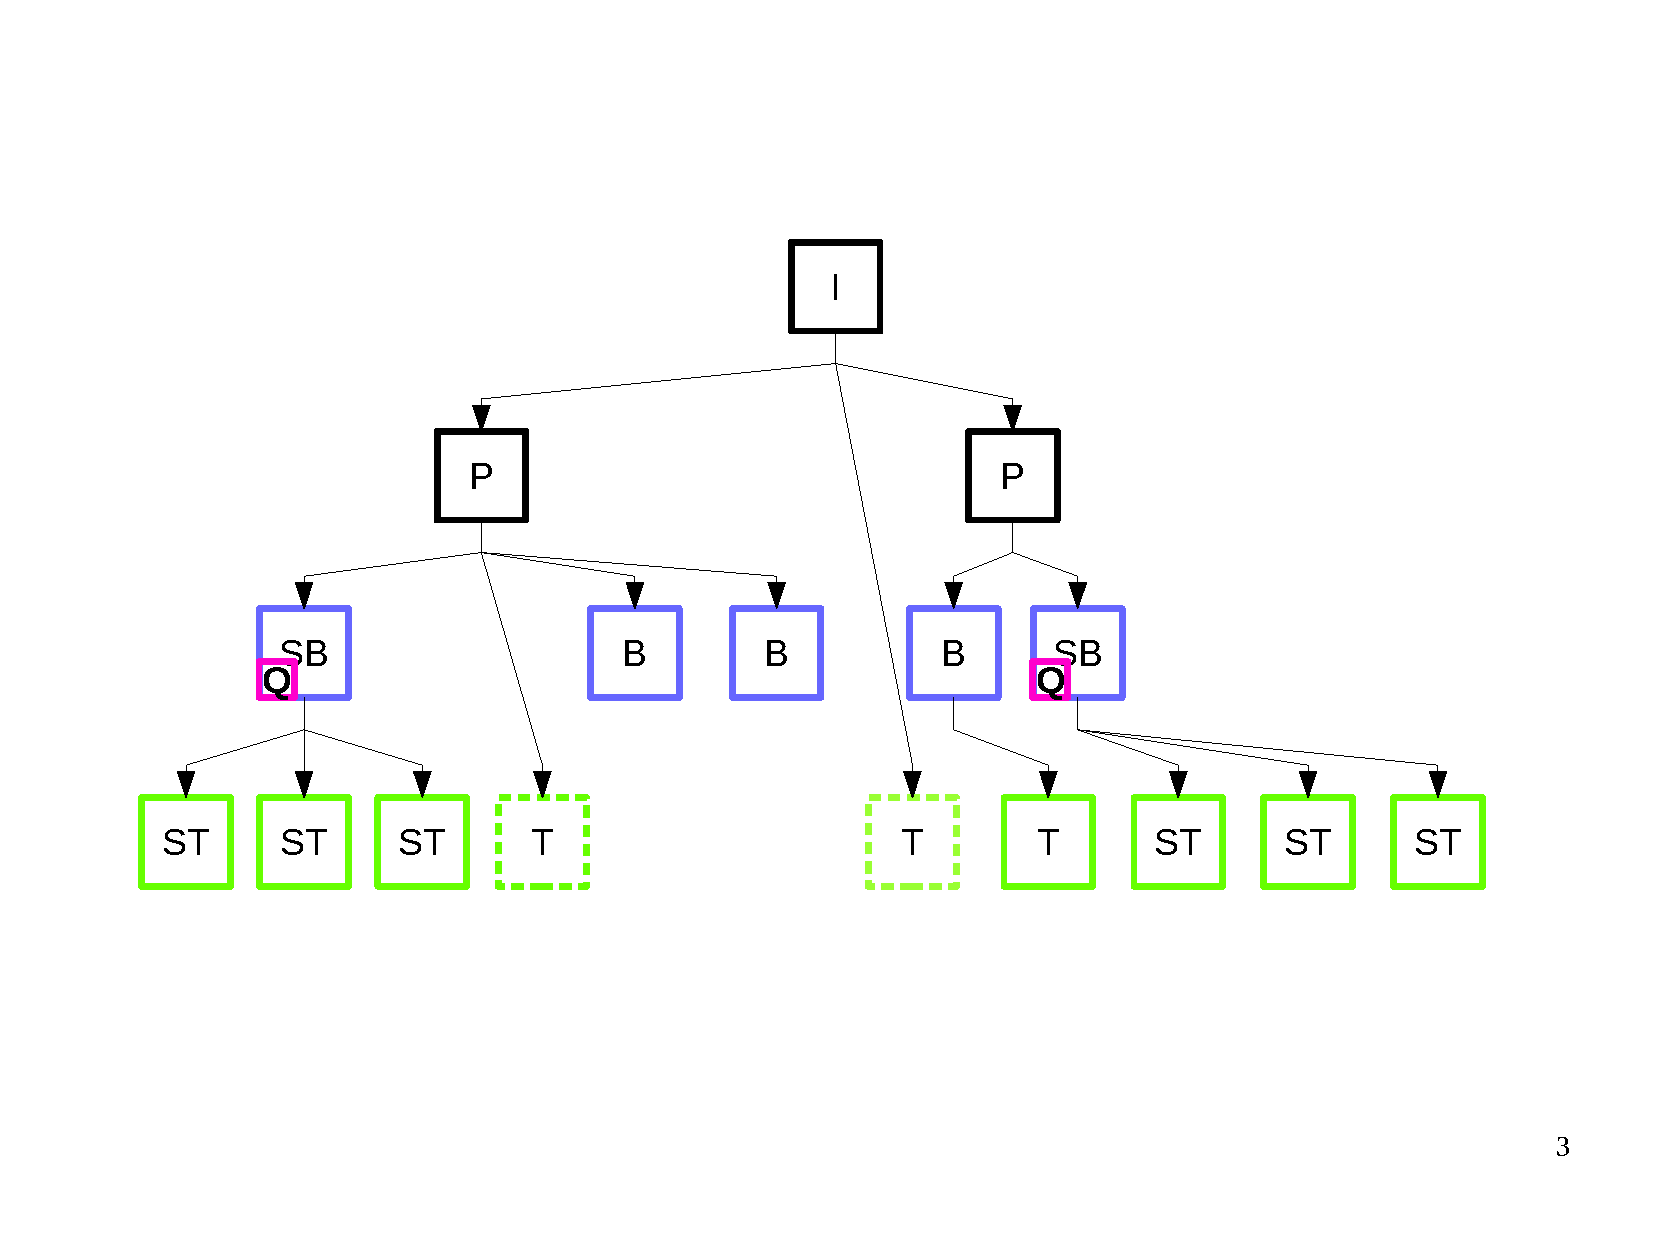
\includegraphics[trim= 30px 168px 20px 110px, clip, width=0.8\textwidth]{graph_infer_1.pdf}
  \caption[Inference of the speech balloon $SB$ and speech text $ST$ regions using the semantic properties of the knowledge base]{Inference of the speech balloon $SB$ and speech text $ST$ regions using the semantic properties of the knowledge base.% Bold edges represent an information spatial and semantic.
  }
  \label{fig:kn:graph_specific_types}
 \end{figure}
%%%%%%%%%%%%%%%%%%%%%%%%%%%%%%%%%%%%%%%%%%%%%%%%%%%

% subsection simple_element_extraction (end)

\subsection{Complex element extraction} % (fold)
\label{sub:complex_element_extraction}

\paragraph{Iteration 2 - step 1 (hypothesis)} % (fold)
\label{par:step_4}
This step is the beginning of the second iteration of the process (Figure~\ref{fig:kn:process_loop}).
At this point the expert system already has some information about the content of the image from which a further hypothesis can be made concerning complex elements such as the region of interest (ROI) of the characters from the speech balloon positions (Figure~\ref{fig:kn:hypothesis_roi}).
The ROIs defined by the expert system are given as seeds to the image processing algorithm (extractor of characters) which in turn feeds the expert system with more precise character locations (Figure~\ref{fig:kn:graph_character_region}).

% Knowing the position of the valid from the valid triplets of panel, text and balloon.
% This is the starting point of the second iteration.

%%%%%%%%%%%%%%%%%%%%%%%%%%%%%%%%%%%%%%%%%%%%%%%%%%%
 \begin{figure}[!ht]  %trim=l b r t  width=0.5\textwidth,
   \centering
   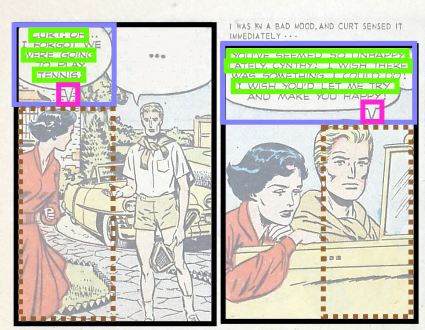
\includegraphics[trim= 0px 0px 0px 0px, clip, width=0.5\textwidth]{process_illustration_hypo_2_1.png}\\
  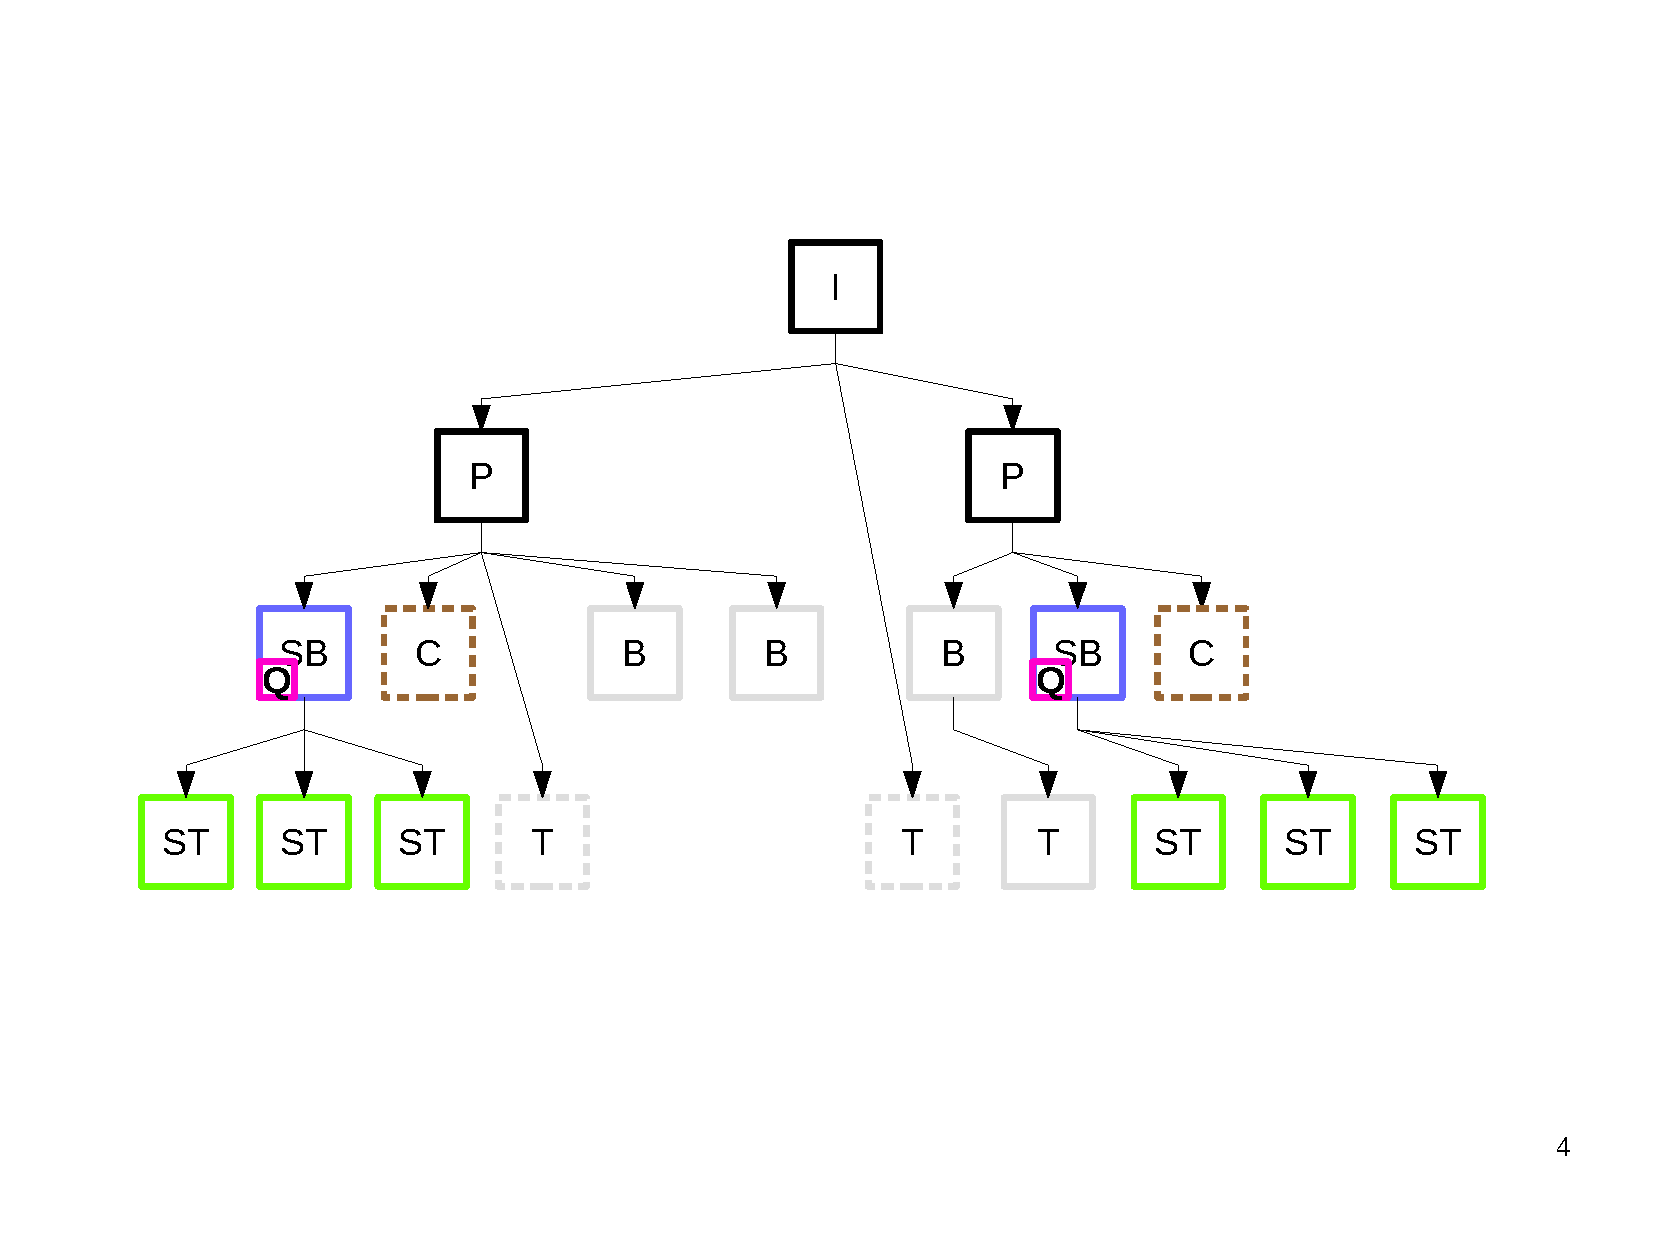
\includegraphics[trim= 30px 168px 20px 110px, clip, width=0.8\textwidth]{graph_init_2_1.pdf}
  \caption[Hypothesis of ROIs of characters $C$ from the speech balloon $SB$ regions and the corresponding image $I$]{Hypothesis of ROIs of characters $C$ from the speech balloon $SB$ regions and the corresponding image $I$. The regions that are not related to $ST$ have been shaded in the graph and removed from the image to make it more comprehensible.
  }
  \label{fig:kn:hypothesis_roi}
 \end{figure}
%%%%%%%%%%%%%%%%%%%%%%%%%%%%%%%%%%%%%%%%%%%%%%%%%%%


%%%%%%%%%%%%%%%%%%%%%%%%%%%%%%%%%%%%%%%%%%%%%%%%%%%
 \begin{figure}[!ht]  %trim=l b r t  width=0.5\textwidth,
   \centering
   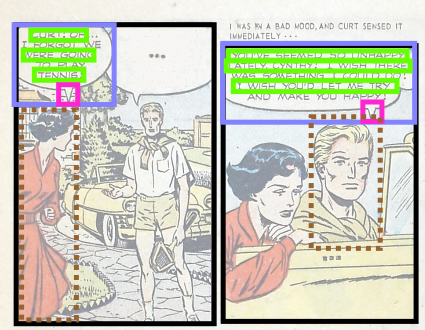
\includegraphics[trim= 0px 0px 0px 0px, clip, width=0.5\textwidth]{process_illustration_hypo_2_2.png}\\
  % 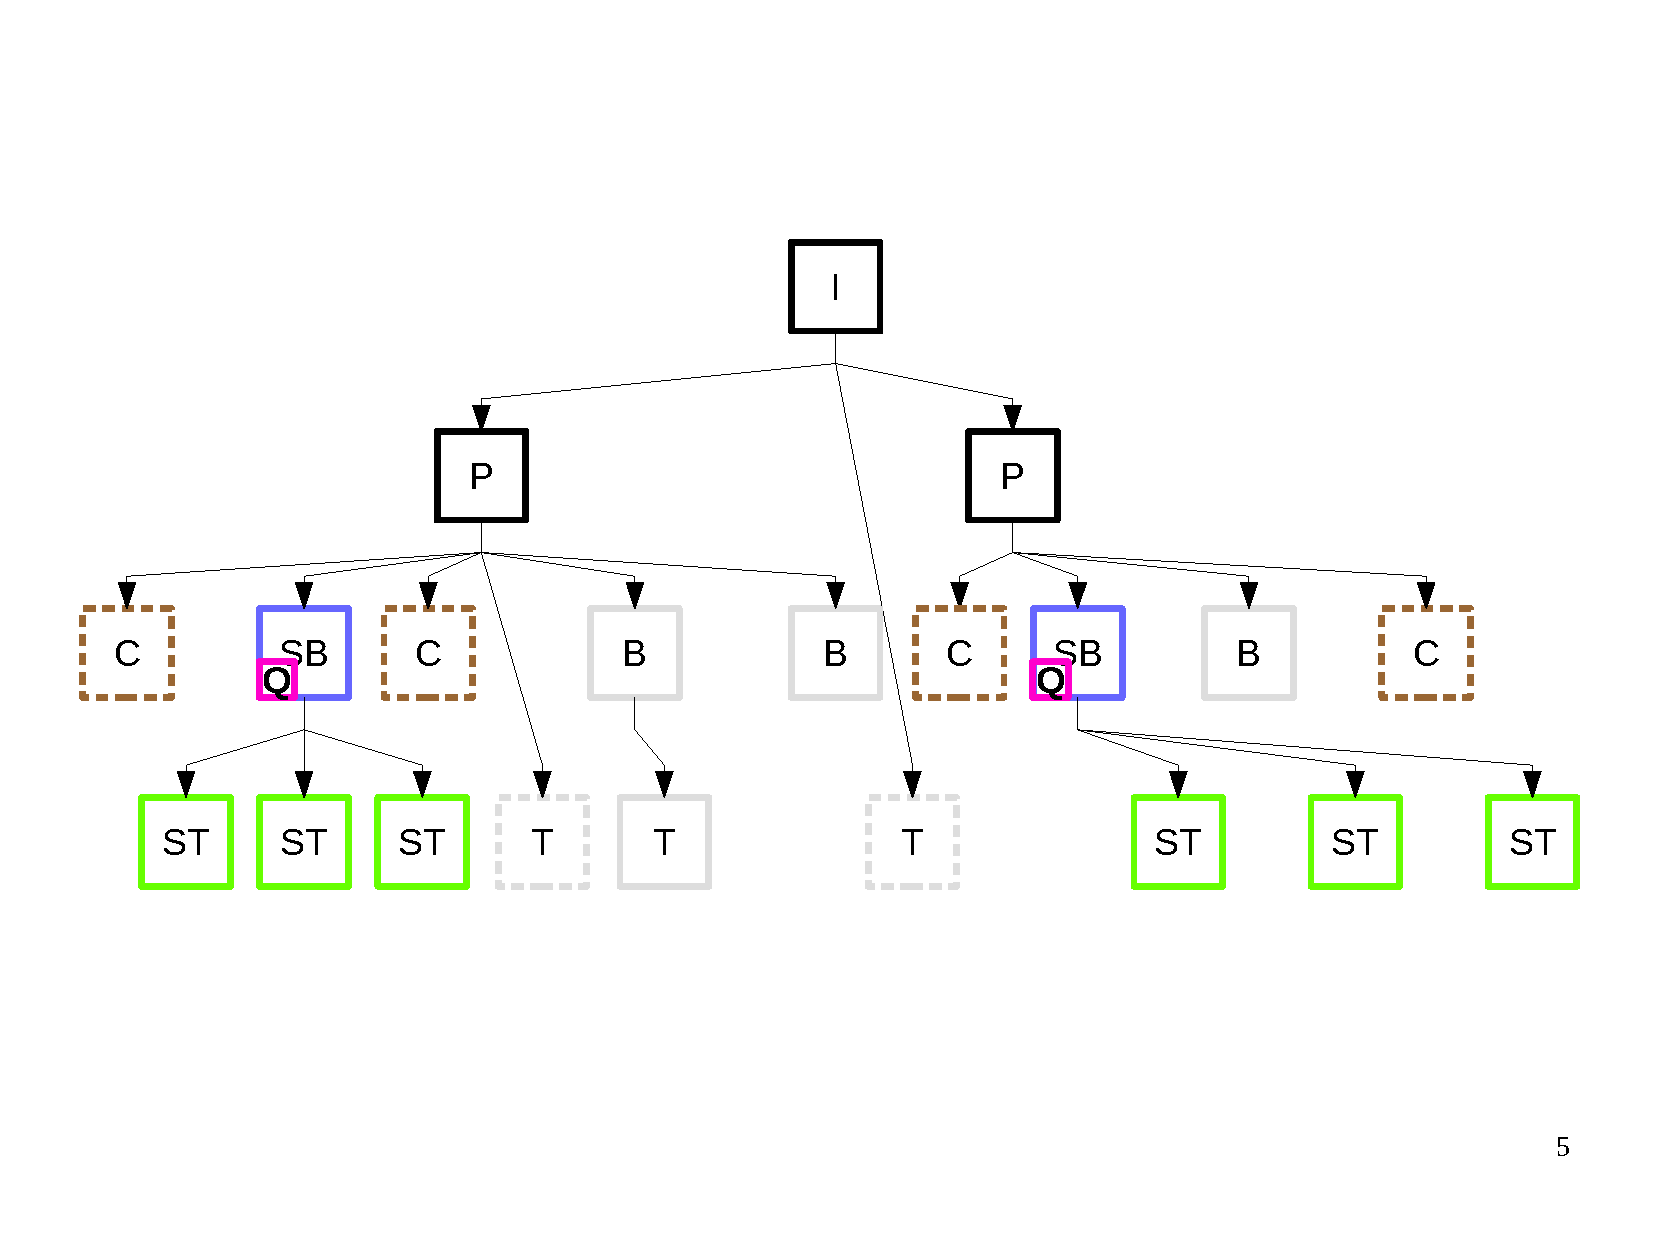
\includegraphics[trim= 0px 168px 20px 85px, clip, width=0.8\textwidth]{fig/graph_init_2_2.pdf}
  \caption[Character locations $C$ returned by the low level processing]{Character locations $C$ returned by the low level processing from the ROIs defined in Figure~\ref{fig:kn:hypothesis_roi}.
  }% added into the graph and the corresponding region in the image $I$.}
  \label{fig:kn:graph_character_region}
 \end{figure}
%%%%%%%%%%%%%%%%%%%%%%%%%%%%%%%%%%%%%%%%%%%%%%%%%%%

\paragraph{Iteration 2 - step 2 (validation)} % (fold)
\label{par:step_5}
The expert system checks if the spatial relations of the characters $C$ match the properties of the knowledge base defined in Section~\ref{sec:kn:constrains_low_level_extraction} (Figure~\ref{fig:kn:valid_2}).


%%%%%%%%%%%%%%%%%%%%%%%%%%%%%%%%%%%%%%%%%%%%%%%%%%%
 \begin{figure}[!ht]  %trim=l b r t  width=0.5\textwidth,
   \centering
   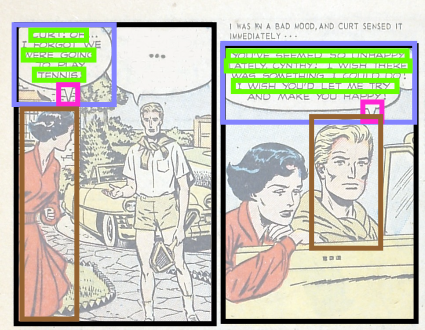
\includegraphics[trim= 0px 0px 0px 0px, clip, width=0.5\textwidth]{process_illustration_valid_2.png}\\
  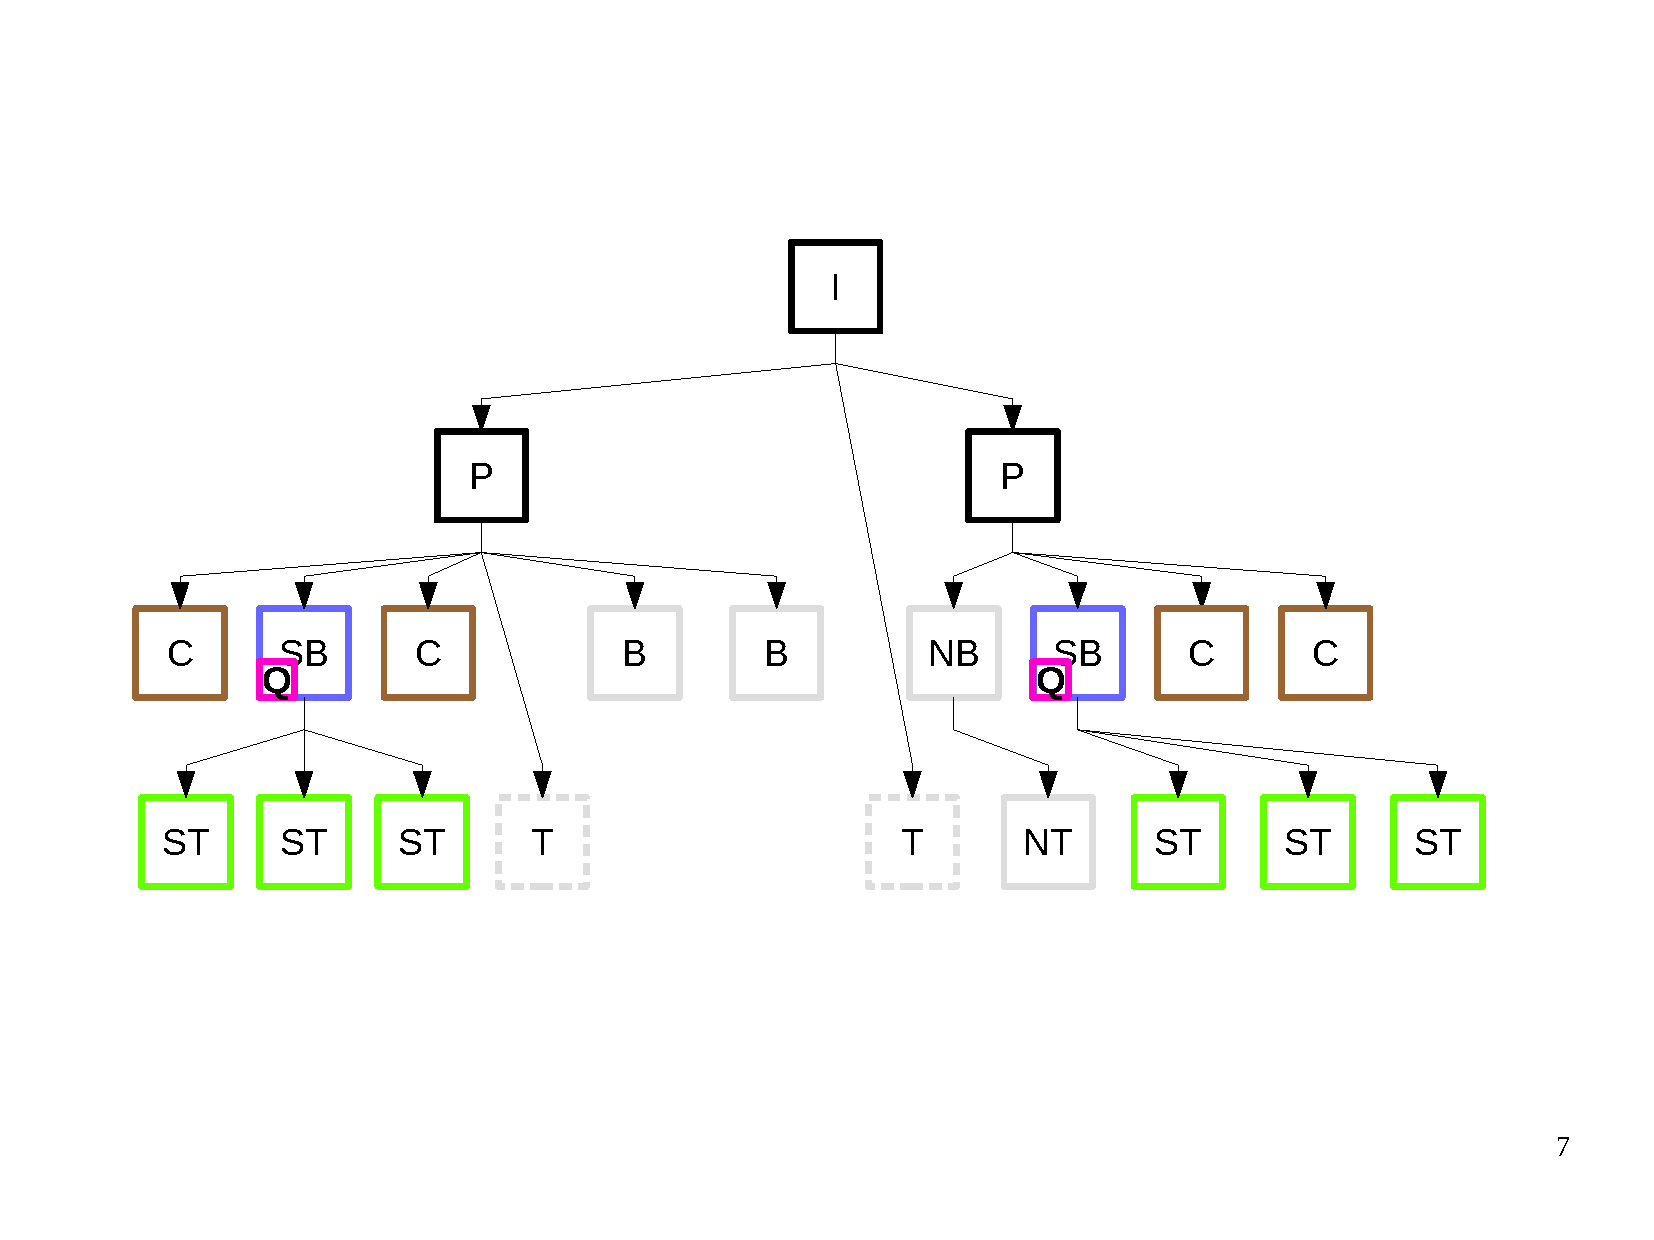
\includegraphics[trim= 0px 128px 20px 85px, clip, width=0.8\textwidth]{graph_valid_2.pdf}
  \caption[Validation of the character regions $C$ by the expert system]{Validation of the character regions $C$ by the expert system and the corresponding image $I$.
  }
  \label{fig:kn:valid_2}
 \end{figure}
%%%%%%%%%%%%%%%%%%%%%%%%%%%%%%%%%%%%%%%%%%%%%%%%%%%

\paragraph{Iteration 2 - step 3 (inference)} % (fold)
\label{par:step_6}
The expert system infers which characters are speaking $SC$ (Section~\ref{sub:inference_of_the_speaking_characters}) and makes a semantic link to the corresponding speech balloons which have already been linked to speech text regions in {\it Iteration 1 - inference} step. (Figure~\ref{fig:kn:final_information}).


%%%%%%%%%%%%%%%%%%%%%%%%%%%%%%%%%%%%%%%%%%%%%%%%%%%
 \begin{figure}[!ht]  %trim=l b r t  width=0.5\textwidth,
   \centering
   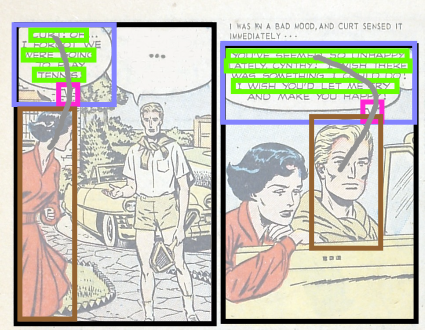
\includegraphics[trim= 0px 0px 0px 0px, clip, width=0.5\textwidth]{process_illustration_infer_2.png}\\
  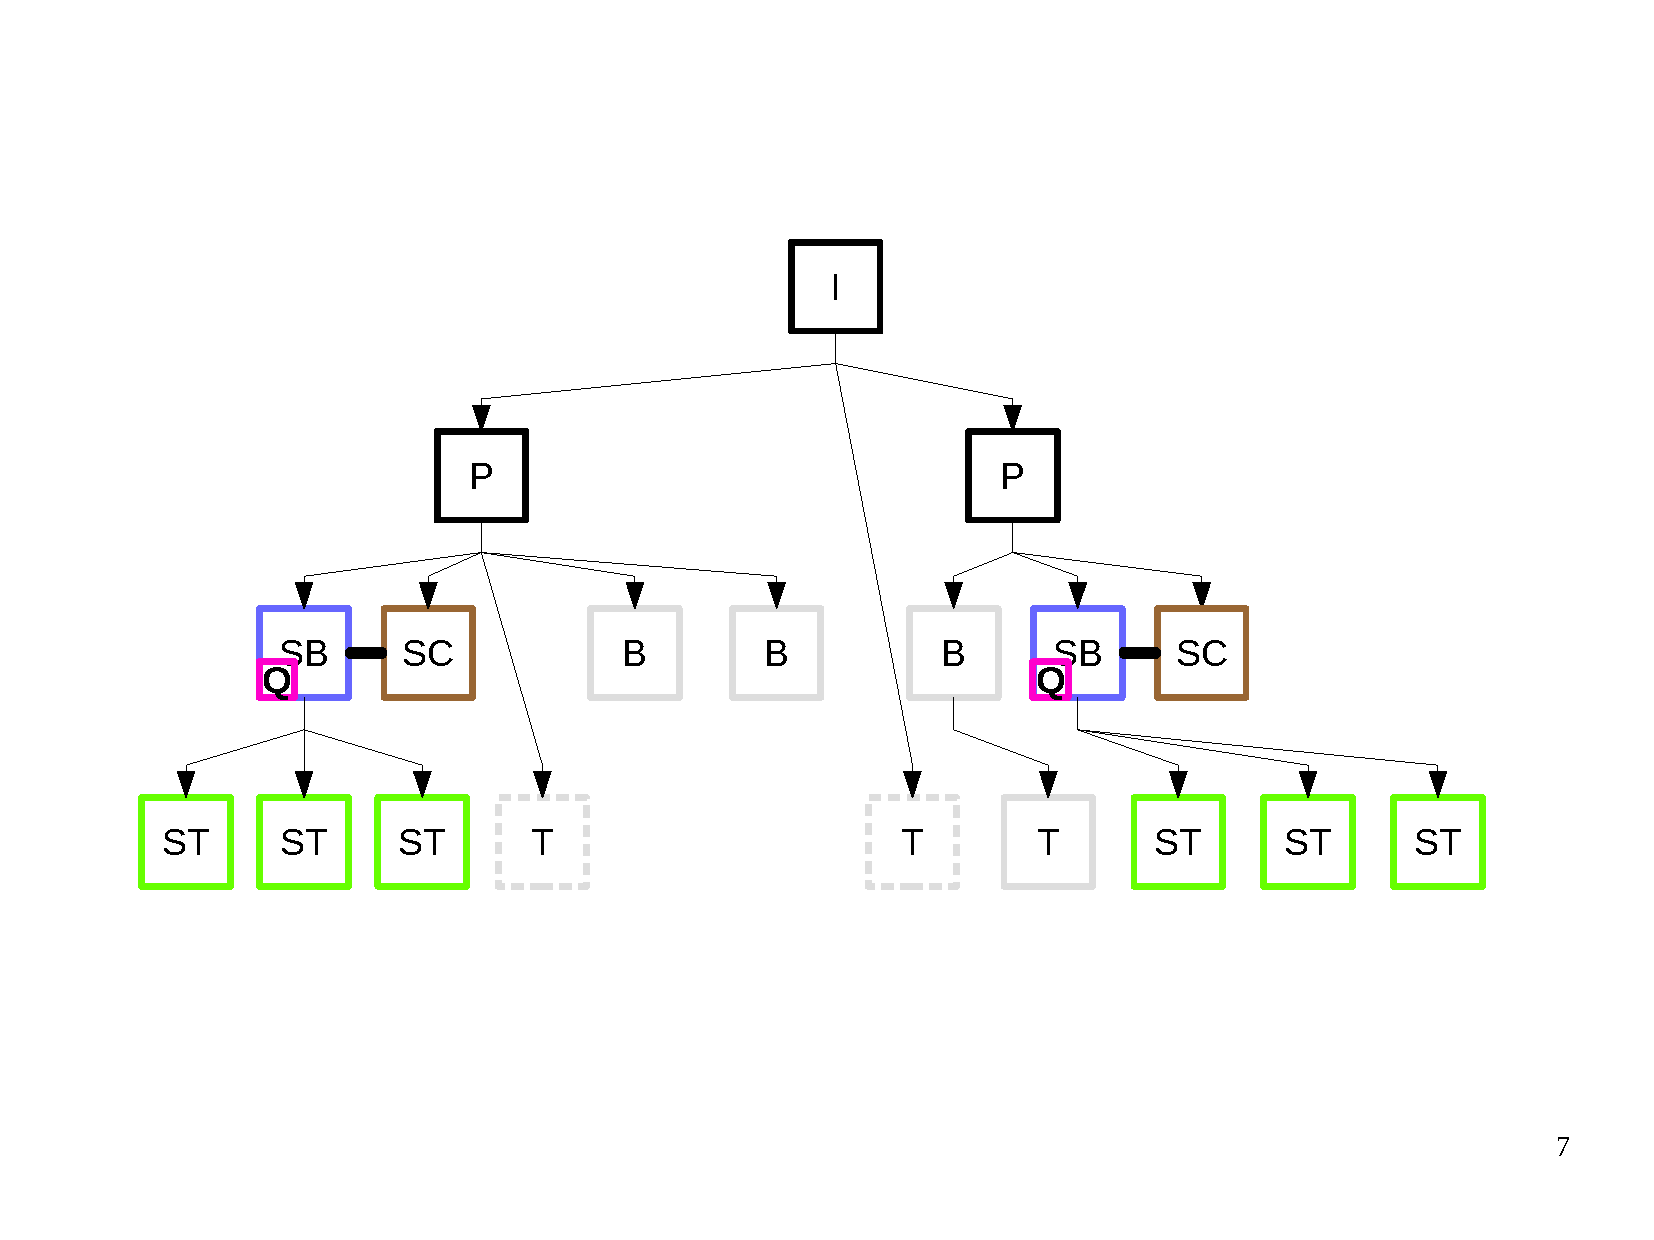
\includegraphics[trim= 0px 128px 20px 85px, clip, width=0.8\textwidth]{graph_infer_2.pdf}
  \caption[Inference of the speaking characters $SC$ and the corresponding semantic links between speaking characters $SC$ and speech balloons $SB$ regions]{Inference of the two speaking characters $SC$ and the corresponding semantic links between speaking characters $SC$ and speech balloons $SB$ regions.
  The two semantic links are represented by a grey stroke in the image over the regions concerned and a non oriented horizontal edge in the graph.
  }
  \label{fig:kn:final_information}
 \end{figure}
%%%%%%%%%%%%%%%%%%%%%%%%%%%%%%%%%%%%%%%%%%%%%%%%%%%

At the end of the two iterations we obtained both a topological and a semantic description of the image content, illustrated here in a single graph here.
Further iteration could be processed by extracting other low level elements such as faces or vehicles and by adding extra domain knowledge.


% subsection complex_element_extraction (end)

% section framework_ (end)

\section{Presentation of the models} % (fold)
\label{sec:kn:model}

The knowledge base is composed of two ontologies, designed using OWL's W3C recommendation~\cite{McGuinness2004}, and interacting with each other (Figure~\ref{fig:kn:generic_expert_system}).
The first one was used to model the raw data provided by image analysis algorithms (called \textit{image model} hereafter), while the second models the comic book domain knowledge (called \textit{comics model}).
These two models are bounded by bridges that are used to perform reasoning over both models, using their own properties.

\subsection{Image model}


\subsection{Comics model}


% \subsection{Model interactions}
% The image and comics models are linked through two bridges.
% First, the \textit{Image} from the image model and \textit{Page} from the comics model concepts are made equivalent by the axiom \texttt{owl:equivalentClass}.
% This way we ensure that all extracted content related to an image is equally related to a corresponding page in the comics domain $Page \equiv  Image$.

% Second, the classes $Cl=\{Panel$, $Balloon$, $TextLine$, $Character\}$ are defined as equivalent to the corresponding set of regions of interest $Sr = \{panels$, $balloons$, $text lines$, $characters\}$ Equation~\ref{eq:kn:class_region_equivalence}).% that have an extractor which purpose is to extract the corresponding panels (resp. balloons, text lines and characters).
	

% \begin{equation}
% \label{eq:kn:class_region_equivalence}
% \begin{split}
% Cl_i  \equiv \text{ROI} \textbf{ and } (hasExtractor \textbf{ some } (roiType \textbf{ value } Sr_i ))
% \end{split}
% \end{equation}

% section model (end)


\section{Interactions between high and low level processing}
\label{sec:kn:interaction_low_high_level_processing}

\modif{TODO: to dispatch in processing sequence subsection}

%This section describes how the extracted data are processed at the semantic level.
This section presents the low and high level processing interaction to validate the extractions, infer information and generate hypotheses about the image content.% we use it to validate the extracted elements, infer more information about them and express region of interest's hypothesis to send back at low-level algorithms.
\subsection{Validation of the extractions} % (fold)
\label{sub:kn:validation}
In order to validate the extraction of the comic page's components, we made sure that the extracted panels, balloons and text lines were in accordance with the knowledge defined in \ref{sec:kn:constrains_low_level_extraction}.
%Those which are not consistent with our model are rejected.

Firstly, each item was loaded into the model as it was labelled (page, panel, balloon, text line or comics character) by the low level processing step.
Then, each element was linked to its smallest container in a half-blind way (Section~\ref{sec:kn:constrains_low_level_extraction}).
That is to say that the type of contained element was known, while the type of  potential container was not.
Not knowing the type of container might have lead to incorrect assertions that would have produced inconsistencies in the model.
Those inconsistencies are the result of possible mistakes made during the extraction process that were filtered out in order to improve the overall detection precision.
Consistency checking was performed over the model and inconsistencies were handled one after the other.
We chose to focus on increasing the extraction precision by deleting those elements that did not fit the constrained model.
The detection of misclassified elements (a panel actually being a balloon) and the proposition of missed elements (like a missed balloon around a group of text lines) were both perspectives of this work.
For the time being, our system can handled, without being limited to, the following inconsistencies:
%Due to the limited number of object types we deal with, inconsistencies sources can be reduced to this exhaustive list:
\begin{itemize}
	\item \textbf{A page (p) contains a balloon (b), a text line (t) or a character (c)}: b, t or c is deleted.
%	\item \textbf{A page (p) contains a balloon (b)}: if b contains other balloons then b is a panel, otherwise b has to be deleted.
%  	\item \textbf{A page (p) contains a text line (t)}: if t contains other lines then t is a balloon, otherwise t has to be deleted.
	\item \textbf{A panel (p1) contains a panel (p2) or a text line (t)}: p2 or t is deleted.
%  	\item \textbf{A panel (p1) contains a panel (p2)}: if p2 contains any text line then p2 is a balloon, otherwise p2 has to be deleted.
% 	\item \textbf{A panel (p) contains a text line (t)}: if t contains other lines then t is a balloon, otherwise t has to be deleted.
 	\item \textbf{A balloon (b) contains a panel (p)}: if p contains some balloons and b does not contain any text lines, b is deleted, otherwise, p is deleted.
 	%does not contain anything then p is a line, else if p contains any text line then p is a balloon, otherwise b has to be deleted.
	\item \textbf{A balloon (b1) contains a balloon (b2)}: if b1 does not contain any line then b1 is deleted, otherwise b2 is deleted.
	\item \textbf{A balloon (b) contains a character (c)}: c is deleted.
	%\item \textbf{A balloon (b1) contains a balloon (b2)}: if b2 does not contain anything then b2 is a line, else if b1 does not contain any line then b1 is a panel, otherwise b1 has to be deleted.
 	\item \textbf{A text line (t) contains a panel (p)}: if p does not contain any balloon then p is deleted, otherwise t is deleted.
 	\item \textbf{A text line (t) contains a balloon (b)}: if b does not contain any text line then b is deleted, otherwise t is deleted.
	%\item \textbf{A balloon (b1) contains a balloon (b2)}: if b1 does not contain any line then b1 is deleted, otherwise b2 is deleted.
 	\item \textbf{A text line (t1) contains a text line (t2)}: if t1 contains other lines then t1 is deleted, otherwise t2 is deleted.
 	\item \textbf{A text line (t) contains a character (c)}: c is deleted.
 	\item \textbf{A character (c) contains a panel (p), a balloon (b) or a text line (t)}: c is deleted. 	
 	\item \textbf{A character (c1) contains a character (c2)}: c2 is deleted.
\end{itemize}
% subsection validation (end)

\subsection{Inferences from the low level information} % (fold)
\label{sub:inference_from_low_level}

The expert system is able to infer more specific information than that given by the extractors.
For instance, it can deduce which text is spoken or not and which speaking character pronounces the content of which speech balloon.

% % Use of RDFS/OWL (Web ontology language) to model the information domain with the general comics properties listed bellow, base on the type of region given by the low level processing:

% % subsection inference_ (end)

% % \subsection{Region of interest of character (step 4)} % (fold)
% % \label{sub:speaking_region}
% % TO COMPLETE (Clement?)

% The expert system infers the speaking character location from valid speech balloons regions by computing a region from the tail tip to the panel side following the tail direction, for each speech balloon.
% ...
% Those regions are voluntary quite large to maximize the chance to cover at least the speaking characters.

% The regions are passed to the image processing part (character extractor) that will extract all the characters using those regions as seeds.

\paragraph{Speech balloon and speech text} % (fold)
\label{par:speech_balloon_and_speech_text}

The classification of balloons and text respectively into speech balloons and spoken text can be done by running an inference engine on the model (e.g. Racer~\cite{Haarslev2012}] or Pellet~\cite{Sirin2007a}).
To allow reasoning, the model has to be consistent, which is the case after validation step~\ref{sub:kn:validation} when all inconsistencies have been resolved.
In Section~\ref{sec:kn:constrains_low_level_extraction}, we defined a speech balloon as a balloon that has a tail.
In others words, the concept of a \textit{speech balloon} can be seen as a specialization of the \textit{balloon} concept that extends all its properties plus adding a few new ones.
This is expressed in the expert system by defining a property \textit{hasTail} with the constraint that must have a \textit{speech balloon} instance as a source.
Assessing this piece of knowledge, the reasoner will automatically deduce that each instance of \textit{balloon} extended with a \textit{hasTail} property can be specialized into a \textit{speech balloon}.

In a similar way, the concept of \textit{text line} subsumes the concept of \textit{spoken text line}.
It is rendered equivalent to the set of individuals from the \textit{text line} concept that is bound with the property \textit{isLineOf}, which is the inverse property of \textit{hasLine}, to a \textit{speech balloon}.
In other words, the text lines marked as being part of a speech balloon are automatically classified as spoken text lines.


\paragraph{Speaking characters} % (fold)
\label{sub:inference_of_the_speaking_characters}
Among the validated characters (Section~\ref{sub:kn:validation}), we considered as being potential speakers those who intersect with the hypothetical region computed in \ref{sec:se:tail_to_character}.
These regions were computed from each speech balloon, i.e. the balloons that had an identified tail.
An abstract straight line was drawn from that tail tip in the direction indicated by the tail.
The first region of a potential speaker that it touched was considered to be the source of the speech balloon.
This relation was asserted into the ontology with the property \textit{isSaidBy}, between the selected character and the corresponding balloon.
Since the range of this property was set to the concept of \textit{speaking character}, it automatically classified the character instance involved into this class.

% section interaction_low_high_level_processing (end)

% \subsection{Hypothesis} % (fold)
% \label{sub:hypothesis}

% \modif{TODO: ROI same as Method 1, reading order (7.2 Clement), other from Clement's thesis (coming soon)}

% subsection hypothesis (end)

% Conclusion --------------------------------------------------------------------------------------------------------------------------------------
\section{Conclusions}
\label{sec:kn:conclusion}

We presented a new framework for understanding documents that can interact with low and high level information suitable for semi structured and complex background documents such as comics.
Several key improvements to information extraction and processing methods have been developed. 
%We suggest improved methods for panel and balloon extraction along with a first method in the literature to locate the tail tip and the indicated direction by analysing the balloon contour.
We provide a novel generic and unsupervised definition of the comic character region of interest that takes into account the spatial organisation of the rest of the elements in an image.
It relies on an inference engine that interacts with two knowledge models, one for image processing and the other one for comics.
In the future we plan to add more iterations of the process in order to retrieve new information such as spotting the non speaking comic characters using those already detected (speaking characters) for training.
In addition, the expert system will be used to improve text extraction and recognition using system feedback in order to automatically extract open speech balloons from text locations. 

In the next chapter, we are going to experiment the different contributions presented in this thesis and compare them to other methods from the literature.
The dataset is first introduced along with the metrics we used to evaluate information retrieval. 

\modif{
  
Deux ontologies ont été présentées dans ce chapitre, la première formalisant les notions mises en œuvre lors de l'étape d'analyse d'images, l'autre formalisant le domaine de la bande dessinée.

L'ontologie image possède l'avantage d'être totalement indépendante d'un quelconque contexte d'application.
Elle permet de manipuler les données d'entrée à analyser, d'organiser les extractions issues de différents algorithmes et d'en évaluer les performances par rapport à des données de référence.
Le format des concepts représentant les régions d'intérêt et des relations spatiales est compatible avec les standards existants.

L'ontologie BD est composée de concepts permettant de rendre compte de la structure classique d'une bande dessinée.
Cette conceptualisation a été développée dans un objectif d'analyse d'images et s'interface avec l'ontologie image à travers des relations d'équivalence entre certains de leurs concepts.
Nous verrons dans la suite de ce document que certains points peuvent être amendés afin d'adapter tel ou tel aspect du modèle à différents cadres d'application.  
}